% Options for packages loaded elsewhere
\PassOptionsToPackage{unicode}{hyperref}
\PassOptionsToPackage{hyphens}{url}
%
\documentclass[
  a4paper,
]{article}
\usepackage{amsmath,amssymb}
\usepackage{lmodern}
\usepackage{iftex}
\ifPDFTeX
  \usepackage[T1]{fontenc}
  \usepackage[utf8]{inputenc}
  \usepackage{textcomp} % provide euro and other symbols
\else % if luatex or xetex
  \usepackage{unicode-math}
  \defaultfontfeatures{Scale=MatchLowercase}
  \defaultfontfeatures[\rmfamily]{Ligatures=TeX,Scale=1}
\fi
% Use upquote if available, for straight quotes in verbatim environments
\IfFileExists{upquote.sty}{\usepackage{upquote}}{}
\IfFileExists{microtype.sty}{% use microtype if available
  \usepackage[]{microtype}
  \UseMicrotypeSet[protrusion]{basicmath} % disable protrusion for tt fonts
}{}
\makeatletter
\@ifundefined{KOMAClassName}{% if non-KOMA class
  \IfFileExists{parskip.sty}{%
    \usepackage{parskip}
  }{% else
    \setlength{\parindent}{0pt}
    \setlength{\parskip}{6pt plus 2pt minus 1pt}}
}{% if KOMA class
  \KOMAoptions{parskip=half}}
\makeatother
\usepackage{xcolor}
\IfFileExists{xurl.sty}{\usepackage{xurl}}{} % add URL line breaks if available
\IfFileExists{bookmark.sty}{\usepackage{bookmark}}{\usepackage{hyperref}}
\hypersetup{
  pdftitle={MATH5714 Linear Regression, Robustness and Smoothing},
  pdfauthor={Jochen Voss},
  hidelinks,
  pdfcreator={LaTeX via pandoc}}
\urlstyle{same} % disable monospaced font for URLs
\usepackage[margin=1in]{geometry}
\usepackage{color}
\usepackage{fancyvrb}
\newcommand{\VerbBar}{|}
\newcommand{\VERB}{\Verb[commandchars=\\\{\}]}
\DefineVerbatimEnvironment{Highlighting}{Verbatim}{commandchars=\\\{\}}
% Add ',fontsize=\small' for more characters per line
\usepackage{framed}
\definecolor{shadecolor}{RGB}{248,248,248}
\newenvironment{Shaded}{\begin{snugshade}}{\end{snugshade}}
\newcommand{\AlertTok}[1]{\textcolor[rgb]{0.94,0.16,0.16}{#1}}
\newcommand{\AnnotationTok}[1]{\textcolor[rgb]{0.56,0.35,0.01}{\textbf{\textit{#1}}}}
\newcommand{\AttributeTok}[1]{\textcolor[rgb]{0.77,0.63,0.00}{#1}}
\newcommand{\BaseNTok}[1]{\textcolor[rgb]{0.00,0.00,0.81}{#1}}
\newcommand{\BuiltInTok}[1]{#1}
\newcommand{\CharTok}[1]{\textcolor[rgb]{0.31,0.60,0.02}{#1}}
\newcommand{\CommentTok}[1]{\textcolor[rgb]{0.56,0.35,0.01}{\textit{#1}}}
\newcommand{\CommentVarTok}[1]{\textcolor[rgb]{0.56,0.35,0.01}{\textbf{\textit{#1}}}}
\newcommand{\ConstantTok}[1]{\textcolor[rgb]{0.00,0.00,0.00}{#1}}
\newcommand{\ControlFlowTok}[1]{\textcolor[rgb]{0.13,0.29,0.53}{\textbf{#1}}}
\newcommand{\DataTypeTok}[1]{\textcolor[rgb]{0.13,0.29,0.53}{#1}}
\newcommand{\DecValTok}[1]{\textcolor[rgb]{0.00,0.00,0.81}{#1}}
\newcommand{\DocumentationTok}[1]{\textcolor[rgb]{0.56,0.35,0.01}{\textbf{\textit{#1}}}}
\newcommand{\ErrorTok}[1]{\textcolor[rgb]{0.64,0.00,0.00}{\textbf{#1}}}
\newcommand{\ExtensionTok}[1]{#1}
\newcommand{\FloatTok}[1]{\textcolor[rgb]{0.00,0.00,0.81}{#1}}
\newcommand{\FunctionTok}[1]{\textcolor[rgb]{0.00,0.00,0.00}{#1}}
\newcommand{\ImportTok}[1]{#1}
\newcommand{\InformationTok}[1]{\textcolor[rgb]{0.56,0.35,0.01}{\textbf{\textit{#1}}}}
\newcommand{\KeywordTok}[1]{\textcolor[rgb]{0.13,0.29,0.53}{\textbf{#1}}}
\newcommand{\NormalTok}[1]{#1}
\newcommand{\OperatorTok}[1]{\textcolor[rgb]{0.81,0.36,0.00}{\textbf{#1}}}
\newcommand{\OtherTok}[1]{\textcolor[rgb]{0.56,0.35,0.01}{#1}}
\newcommand{\PreprocessorTok}[1]{\textcolor[rgb]{0.56,0.35,0.01}{\textit{#1}}}
\newcommand{\RegionMarkerTok}[1]{#1}
\newcommand{\SpecialCharTok}[1]{\textcolor[rgb]{0.00,0.00,0.00}{#1}}
\newcommand{\SpecialStringTok}[1]{\textcolor[rgb]{0.31,0.60,0.02}{#1}}
\newcommand{\StringTok}[1]{\textcolor[rgb]{0.31,0.60,0.02}{#1}}
\newcommand{\VariableTok}[1]{\textcolor[rgb]{0.00,0.00,0.00}{#1}}
\newcommand{\VerbatimStringTok}[1]{\textcolor[rgb]{0.31,0.60,0.02}{#1}}
\newcommand{\WarningTok}[1]{\textcolor[rgb]{0.56,0.35,0.01}{\textbf{\textit{#1}}}}
\usepackage{longtable,booktabs,array}
\usepackage{calc} % for calculating minipage widths
% Correct order of tables after \paragraph or \subparagraph
\usepackage{etoolbox}
\makeatletter
\patchcmd\longtable{\par}{\if@noskipsec\mbox{}\fi\par}{}{}
\makeatother
% Allow footnotes in longtable head/foot
\IfFileExists{footnotehyper.sty}{\usepackage{footnotehyper}}{\usepackage{footnote}}
\makesavenoteenv{longtable}
\usepackage{graphicx}
\makeatletter
\def\maxwidth{\ifdim\Gin@nat@width>\linewidth\linewidth\else\Gin@nat@width\fi}
\def\maxheight{\ifdim\Gin@nat@height>\textheight\textheight\else\Gin@nat@height\fi}
\makeatother
% Scale images if necessary, so that they will not overflow the page
% margins by default, and it is still possible to overwrite the defaults
% using explicit options in \includegraphics[width, height, ...]{}
\setkeys{Gin}{width=\maxwidth,height=\maxheight,keepaspectratio}
% Set default figure placement to htbp
\makeatletter
\def\fps@figure{htbp}
\makeatother
\setlength{\emergencystretch}{3em} % prevent overfull lines
\providecommand{\tightlist}{%
  \setlength{\itemsep}{0pt}\setlength{\parskip}{0pt}}
\setcounter{secnumdepth}{5}
\ifLuaTeX
  \usepackage{selnolig}  % disable illegal ligatures
\fi
\usepackage[]{natbib}
\bibliographystyle{plainnat}

\title{MATH5714 Linear Regression, Robustness and Smoothing}
\author{\href{mailto:J.Voss@leeds.ac.uk}{Jochen Voss}}
\date{University of Leeds, Semester 1, 2021--22}

\usepackage{amsthm}
\newtheorem{theorem}{Theorem}[section]
\newtheorem{lemma}{Lemma}[section]
\newtheorem{corollary}{Corollary}[section]
\newtheorem{proposition}{Proposition}[section]
\newtheorem{conjecture}{Conjecture}[section]
\theoremstyle{definition}
\newtheorem{definition}{Definition}[section]
\theoremstyle{definition}
\newtheorem{example}{Example}[section]
\theoremstyle{definition}
\newtheorem{exercise}{Exercise}[section]
\theoremstyle{definition}
\newtheorem{hypothesis}{Hypothesis}[section]
\theoremstyle{remark}
\newtheorem*{remark}{Remark}
\newtheorem*{solution}{Solution}
\begin{document}
\maketitle

{
\setcounter{tocdepth}{2}
\tableofcontents
}
\newcommand{\argmin}{\mathop{\mathrm{arg\,min}}\limits}
\newcommand{\bias}{\mathop{\mathrm{bias}}}
\newcommand{\CN}{\mathcal{N}}
\newcommand{\CU}{\mathcal{U}}
\newcommand{\downto}{\downarrow}
\newcommand{\ds}{\displaystyle}
\newcommand{\E}{\mathbb{E}}
\newcommand{\eps}{\varepsilon}
\newcommand{\MSE}{\mathop{\mathrm{MSE}}\nolimits}
\newcommand{\N}{\mathbb{N}}
\renewcommand{\phi}{\varphi}
\newcommand{\R}{\mathbb{R}}
\newcommand{\Var}{\mathop{\mathrm{Var}}}

\hypertarget{home}{%
\section*{Preface}\label{home}}
\addcontentsline{toc}{section}{Preface}

From previous modules we know how to fit a regression line through
points \((x_1, y_1), \ldots, (x_n, y_n) \in\mathbb{R}^2\). The underlying model
here is described by the equation
\begin{equation*}
  y_i
  = \alpha + \beta x_i + \varepsilon_i
\end{equation*}
for all \(i \in \{1, 2, \ldots, n\}\), and the aim is to find values for
the intercept \(\alpha\) and the slope \(\beta\) such that the residuals
\(\varepsilon_i\) are as small as possible. This procedure,
linear regression, and its extensions are discussed in the \href{https://seehuhn.github.io/MATH3714/}{level 3
component of the module}.

In the level 5 component of this module, we will discuss ``smoothing''
which is a technique which can be used when linear models are no longer
appropriate for the data. An example of such a situation is illustrated
in figure~\ref{fig:accel}.



\begin{figure}

{\centering 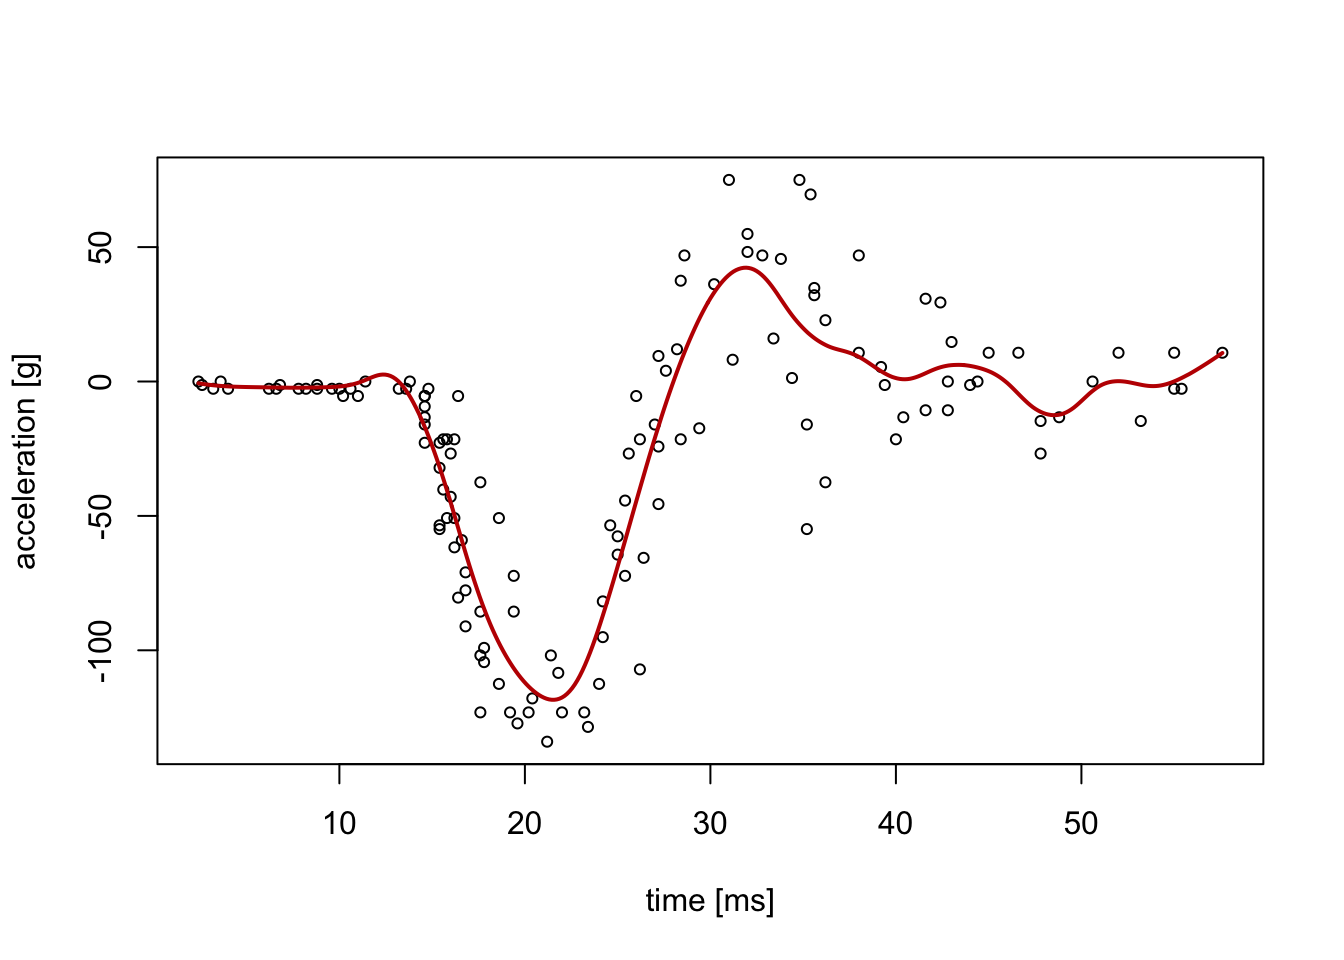
\includegraphics{MATH5714M_files/figure-latex/accel-1} 

}

\caption{An illustration of a data set where a linear (straight line) model is not appropriate. The data represents a series of measurements of head acceleration in a simulated motorcycle accident, used to test crash helmets (the \texttt{mcycle} dataset from the \texttt{MASS} R package).}\label{fig:accel}
\end{figure}

\clearpage

\hypertarget{X01-KDE}{%
\section{Kernel Density Estimation}\label{X01-KDE}}

In this section we discuss the topic of ``Kernel Density Estimation''.
Here we suppose we are given data \(x_1,\ldots, x_n \in\mathbb{R}^d\) from an
unknown probability density, say \(f\). Our objective is to estimate
the density~\(f\). This section lays the foundations for many of the
following topics.

\hypertarget{histograms}{%
\subsection{Histograms}\label{histograms}}

\hypertarget{probability-densities}{%
\subsubsection{Probability Densities}\label{probability-densities}}

Before we consider how to estimate a density, let just remember what a
density is. A random variable \(X \in \mathbb{R}\) has \textbf{density} \(f\colon \mathbb{R}\to [0, \infty)\) if
\begin{equation*}
  P\bigl(X \in [a,b]\bigr)
  = \int_a^b f(x) \,dx
\end{equation*}
for all \(a, b\in\mathbb{R}\) with \(a < b\). Densities are sometimes also called
``probability densities'' or even ``probability density functions''.

A density \(f\) is large in regions where \(X\) is very likely to take
values, and small in regions where \(X\) is less likely to take values.
If \(f(x) = 0\) for all \(x\) in a region, that means that \(X\) never takes
values there. Graphically, the integral \(\int_a^b f(x) \,dx\) can be
interpreted as the area under the graph of~\(f\). This is illustrated
in figure~\ref{fig:density}.



\begin{figure}

{\centering 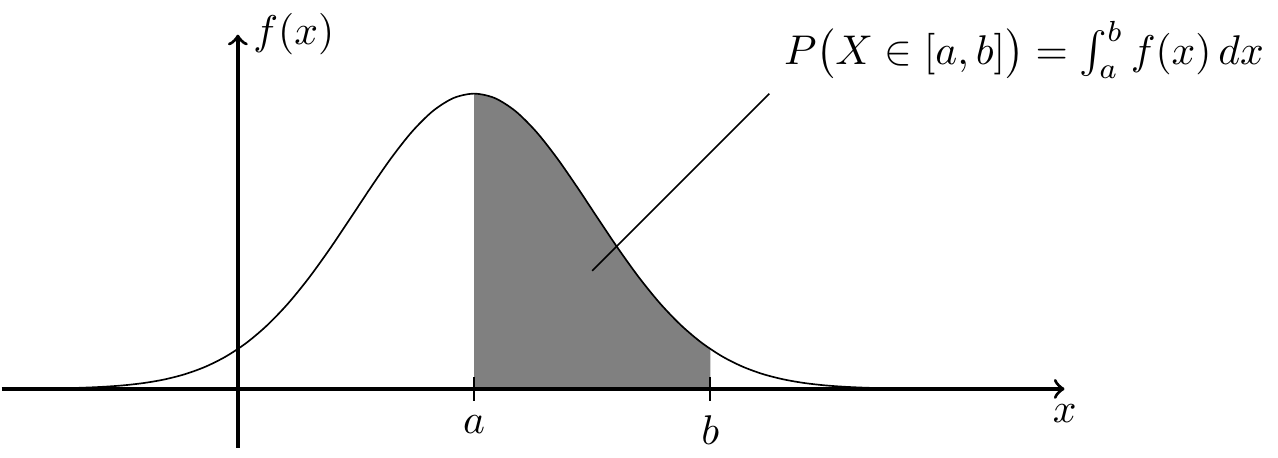
\includegraphics{MATH5714M_files/figure-latex/density-1} 

}

\caption{An illustration of how the area under the graph of a density can be interpreted as a probability.}\label{fig:density}
\end{figure}

A function \(f\) is the density of some random variable~\(X\),
if and only if \(f \geq 0\) and
\begin{equation*}
  \int_{-\infty}^\infty f(x) \,dx = 1.
\end{equation*}

\hypertarget{histograms-1}{%
\subsubsection{Histograms}\label{histograms-1}}

In the univariate case, \emph{i.e.}~for \(d = 1\), a commonly used technique
to approximate density of a sample is to plot a histogram. To
illustrate this, we use the \texttt{faithful} dataset built in R, which
contains waiting times between eruptions and the duration of the
eruption for the Old Faithful geyser in the Yellowstone National Park.
(You can type \texttt{help(faithful)} in R to learn more about this data
set.) Here we focus on the waiting times only. A simple histogram
for this dataset is shown in figure~\ref{fig:hist}.



\begin{Shaded}
\begin{Highlighting}[]
\NormalTok{x }\OtherTok{\textless{}{-}}\NormalTok{ faithful}\SpecialCharTok{$}\NormalTok{waiting}
\FunctionTok{hist}\NormalTok{(x, }\AttributeTok{probability =} \ConstantTok{TRUE}\NormalTok{,}
     \AttributeTok{main =} \ConstantTok{NULL}\NormalTok{, }\AttributeTok{xlab =} \StringTok{"time between eruptions [mins]"}\NormalTok{)}
\end{Highlighting}
\end{Shaded}

\begin{figure}
\centering
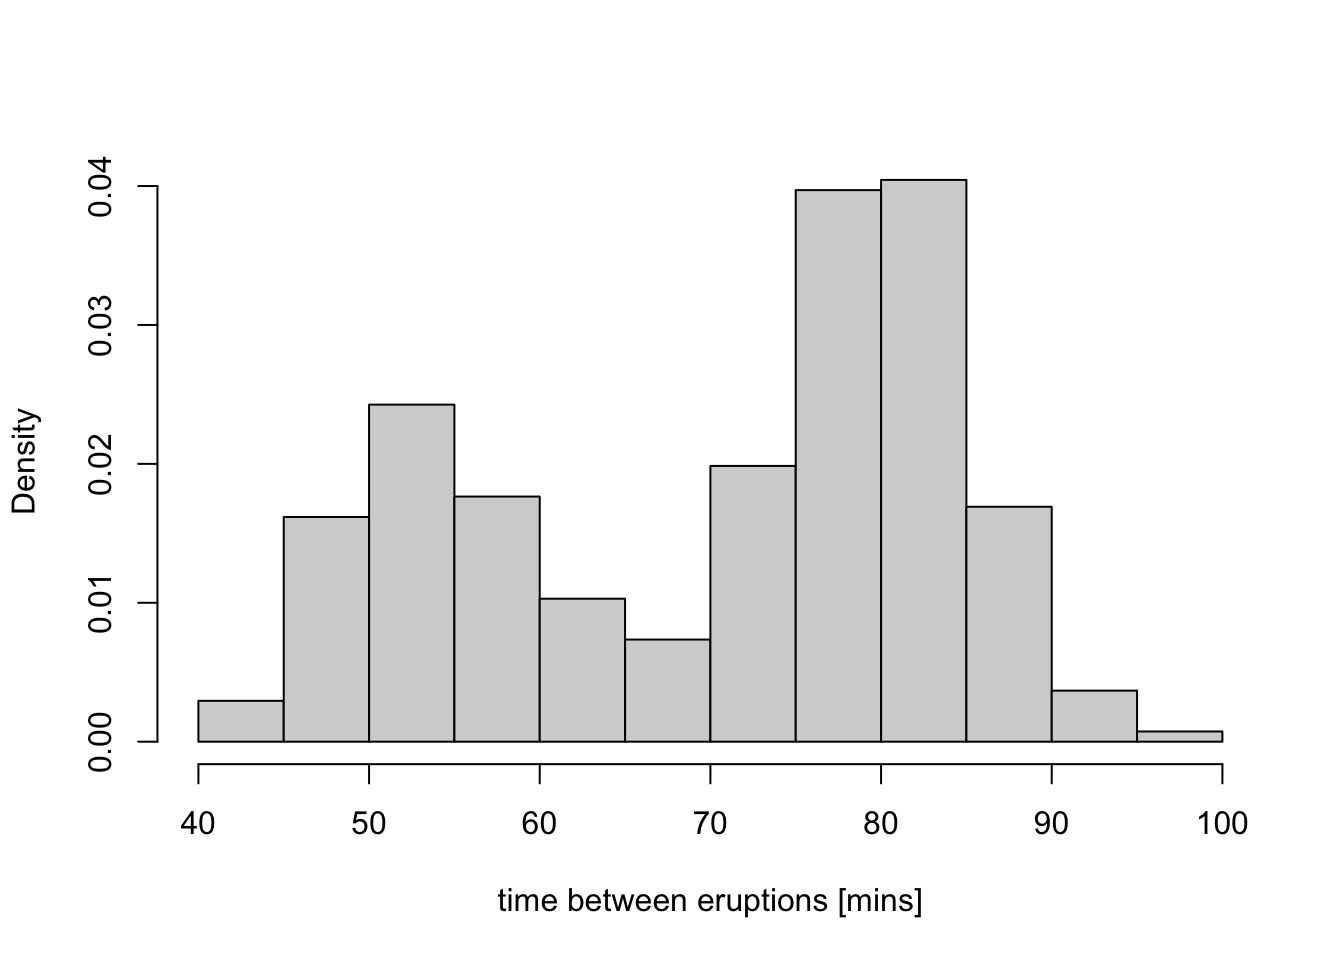
\includegraphics{MATH5714M_files/figure-latex/hist-1.pdf}
\caption{\label{fig:hist}This figure shows how a histogram can be used to approximate a probability density. From the plot one can see that the density of the waiting times distribution seems to be bi-modal with peaks around 53 and 80 minutes.}
\end{figure}

The histograms splits the range of the data into ``buckets'', and for
every bucket \([a, b]\) it shows a bar where the height is proportional
the number of samples in the bucket. I am ignoring the case that a
sample may fall exactly on the boundary between two buckets here; in
reality all but one buckets need to be half-open intervals, for
example \([40, 45]\), \((45, 50]\), \ldots, \((95, 100]\).

As we have seen, the area under the graph of the density \(f\) over the
interval \([a, b]\) corresponds to the probability~\(P\bigl(X \in [a,b]\bigr)\). For the histogram to approximate the density, we need
to scale the height \(h_{a,b}\) of the bucket \([a, b]\) so that the area
in the histogram is also close to this probability. Since we don't
know the probability \(P\bigl(X \in [a,b]\bigr)\) exactly, we have to
approximate it as
\begin{equation*}
  P\bigl(X \in [a,b]\bigr)
  \approx \frac{n_{a,b}}{n},
\end{equation*}
where \(n_{a,b}\) is the number of samples in the bucket \([a,b]\),
and \(n\) is the total number of samples. So we need
\begin{align*}
  (b-a) \cdot h_{a,b}
    &= \mbox{area of the histogram bar} \\
    &\approx \mbox{area of the density} \\
    &= P\bigl(X \in [a,b]\bigr) \\
    &\approx \frac{n_{a,b}}{n}.
\end{align*}
and thus we choose
\begin{equation*}
  h_{a,b}
  = \frac{1}{(b - a) n} n_{a,b}.
\end{equation*}
As expected, the height of the bar for the bucket \([a,b]\) is proportional
to the number \(n_{a,b}\) of samples in the bucket.

\hypertarget{choice-of-buckets}{%
\subsubsection{Choice of Buckets}\label{choice-of-buckets}}

Histograms are only meaningful if the buckets are chosen well. If
the buckets are too large, not much of the structure of \(f\) can be
resolved. If the buckets are too small, the estimate \(P\bigl(X \in [a,b]\bigr) \approx n_{a,b}/n\) will be poor and the histogram will
no longer resemble the shape of~\(f\). This



\begin{Shaded}
\begin{Highlighting}[]
\FunctionTok{set.seed}\NormalTok{(}\DecValTok{1}\NormalTok{)}
\NormalTok{x }\OtherTok{\textless{}{-}} \FunctionTok{rnorm}\NormalTok{(}\DecValTok{50}\NormalTok{)}
\FunctionTok{hist}\NormalTok{(x, }\AttributeTok{probability =} \ConstantTok{TRUE}\NormalTok{, }\AttributeTok{main =} \ConstantTok{NULL}\NormalTok{,}
     \AttributeTok{breaks =} \FunctionTok{seq}\NormalTok{(}\SpecialCharTok{{-}}\FloatTok{2.5}\NormalTok{, }\FloatTok{2.5}\NormalTok{, }\AttributeTok{length.out =} \DecValTok{500}\NormalTok{))}
\end{Highlighting}
\end{Shaded}

\begin{figure}
\centering
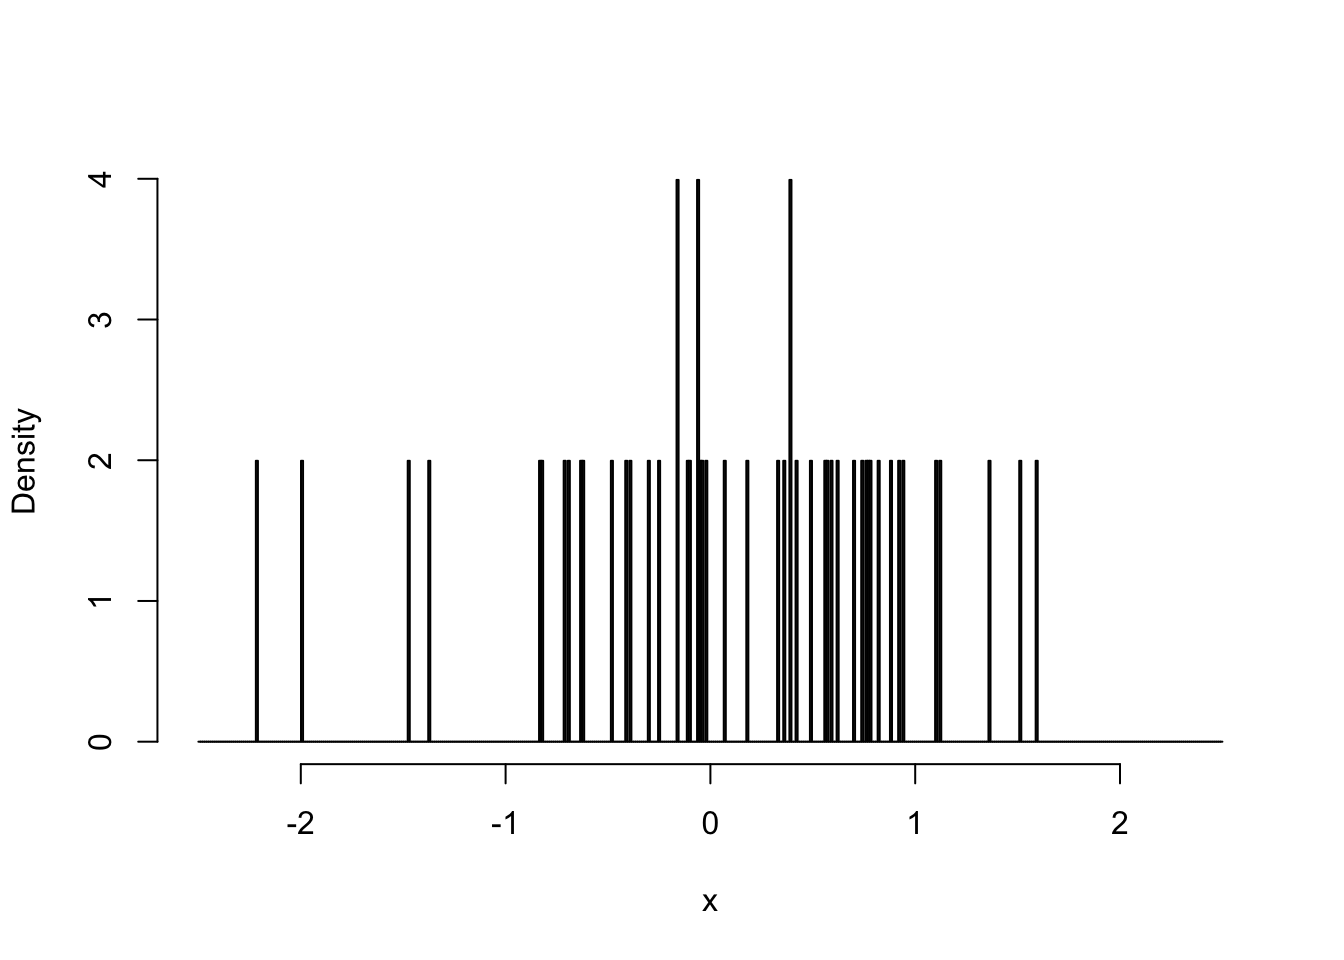
\includegraphics{MATH5714M_files/figure-latex/broken-hist-1.pdf}
\caption{\label{fig:broken-hist}This figure shows how a histogram can be used to approximate a probability density. From the plot one can see that the density of the waiting times distribution seems to be bi-modal with peaks around 53 and 80 minutes.}
\end{figure}

Finally, even if reasonable bucket sizes are chosen, the result can
depend quite strongly on the exact locations of these buckets. To illustrate
this effect, we consider a
(dataset about the annual amount of snow){[}\url{https://teaching.seehuhn.de/data/buffalo/}{]}
falling in Buffalo, New York for different years. Figures \ref{fig:buffalo1}
and~\ref{fig:buffalo2} show that same data in two different ways,
allowing to come to different conclusions about the distribution.



\begin{Shaded}
\begin{Highlighting}[]
\CommentTok{\# downloaded from https://teaching.seehuhn.de/data/buffalo/}
\NormalTok{x }\OtherTok{\textless{}{-}} \FunctionTok{read.csv}\NormalTok{(}\StringTok{"data/buffalo.csv"}\NormalTok{)}
\NormalTok{snowfall }\OtherTok{\textless{}{-}}\NormalTok{ x}\SpecialCharTok{$}\NormalTok{snowfall}
\FunctionTok{hist}\NormalTok{(snowfall, }\AttributeTok{probability =} \ConstantTok{TRUE}\NormalTok{,}
     \AttributeTok{breaks =} \FunctionTok{seq}\NormalTok{(}\FloatTok{24.30}\NormalTok{, }\FloatTok{208.22}\NormalTok{, }\AttributeTok{length.out =} \DecValTok{20}\NormalTok{),}
     \AttributeTok{main =} \ConstantTok{NULL}\NormalTok{, }\AttributeTok{xlab =} \StringTok{"snowfall [in]"}\NormalTok{)}
\end{Highlighting}
\end{Shaded}

\begin{figure}
\centering
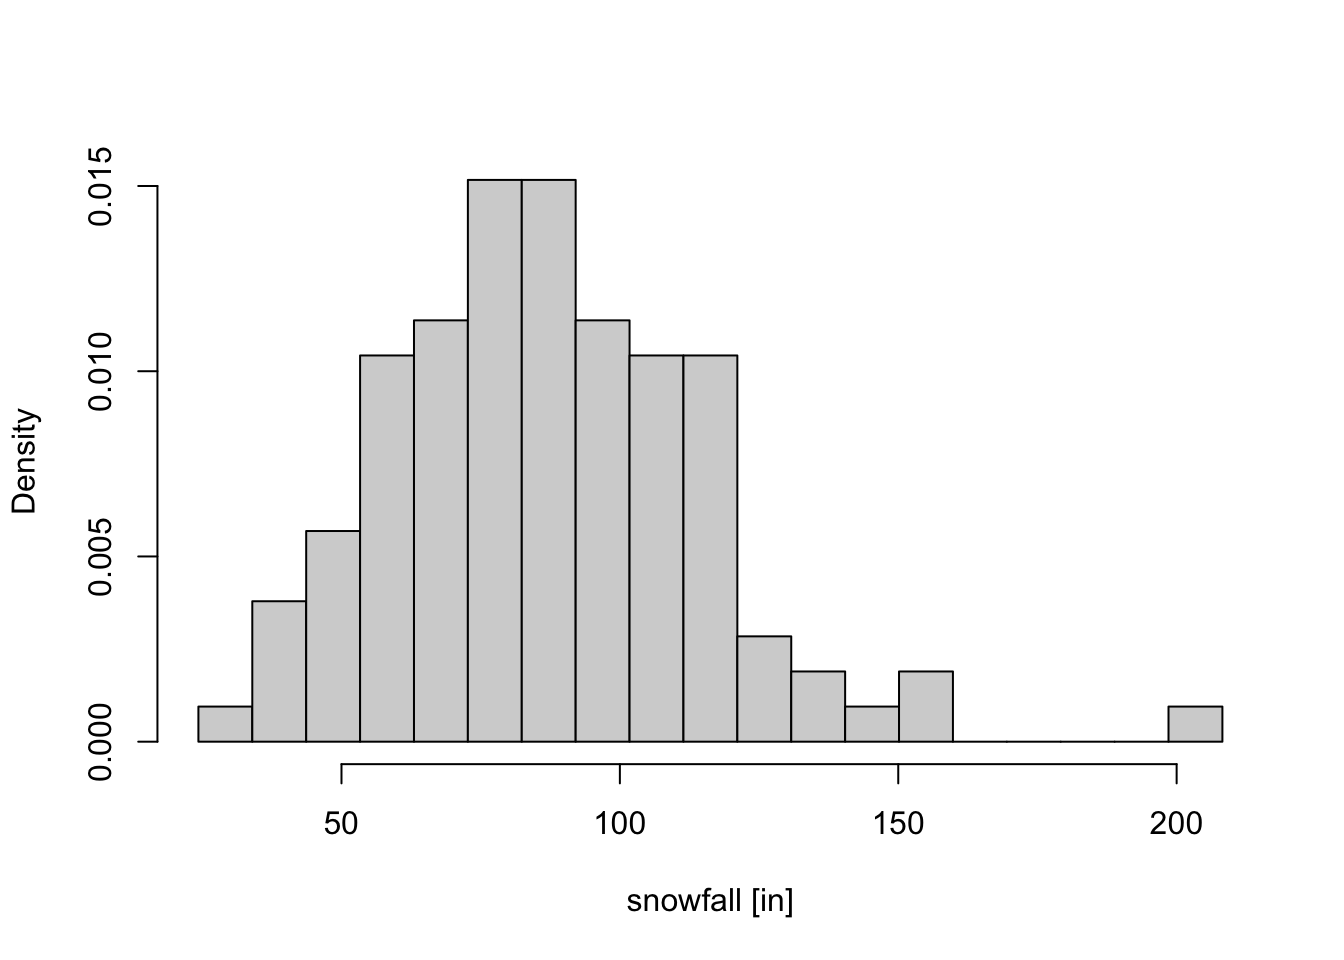
\includegraphics{MATH5714M_files/figure-latex/buffalo1-1.pdf}
\caption{\label{fig:buffalo1}The annual amount of snowfall in Buffalo, New York, in inches. The histogram makes it plausible that there is one main peak in the distribution.}
\end{figure}



\begin{Shaded}
\begin{Highlighting}[]
\FunctionTok{hist}\NormalTok{(snowfall, }\AttributeTok{probability =} \ConstantTok{TRUE}\NormalTok{,}
     \AttributeTok{breaks =} \FunctionTok{seq}\NormalTok{(}\FloatTok{22.85}\NormalTok{, }\FloatTok{204.92}\NormalTok{, }\AttributeTok{length.out =} \DecValTok{20}\NormalTok{),}
     \AttributeTok{main =} \ConstantTok{NULL}\NormalTok{, }\AttributeTok{xlab =} \StringTok{"snowfall [in]"}\NormalTok{)}
\end{Highlighting}
\end{Shaded}

\begin{figure}
\centering
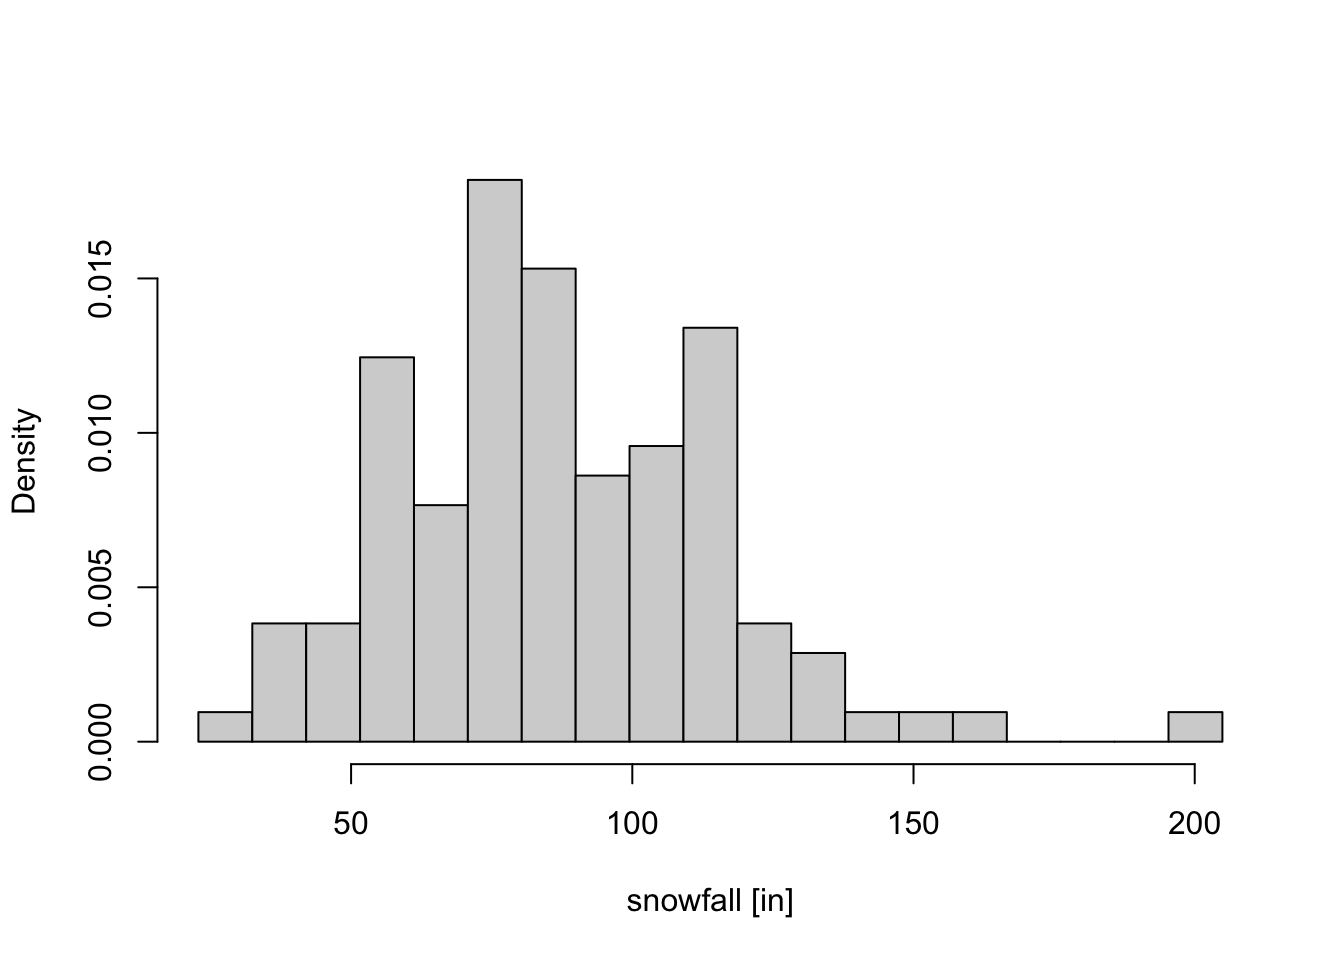
\includegraphics{MATH5714M_files/figure-latex/buffalo2-1.pdf}
\caption{\label{fig:buffalo2}Continued from \ref{fig:buffalo1}, this histogram shows the dataset in a way that three peaks are visible.}
\end{figure}

As a further illustration of the effect of bucket width, the code in
figure~\ref{fig:snow-hist-col} shows how histograms with different
bucket widths can be generated in~R. Here we simply specify numeric
values for the \texttt{break} argument to \texttt{hist()}, which R uses as the
\emph{approximate} number of buckets in the plot.



\begin{Shaded}
\begin{Highlighting}[]
\FunctionTok{par}\NormalTok{(}\AttributeTok{mfrow =} \FunctionTok{c}\NormalTok{(}\DecValTok{2}\NormalTok{,}\DecValTok{2}\NormalTok{))}

\ControlFlowTok{for}\NormalTok{ (breaks }\ControlFlowTok{in} \FunctionTok{c}\NormalTok{(}\DecValTok{80}\NormalTok{, }\DecValTok{40}\NormalTok{, }\DecValTok{20}\NormalTok{, }\DecValTok{10}\NormalTok{)) \{}
  \FunctionTok{hist}\NormalTok{(snowfall,}
       \AttributeTok{prob =} \ConstantTok{TRUE}\NormalTok{,}
       \AttributeTok{breaks =}\NormalTok{ breaks,}
       \AttributeTok{xlim =} \FunctionTok{c}\NormalTok{(}\DecValTok{25}\NormalTok{,}\DecValTok{200}\NormalTok{),}
       \AttributeTok{ylim =} \FunctionTok{c}\NormalTok{(}\DecValTok{0}\NormalTok{, }\FloatTok{0.03}\NormalTok{),}
       \AttributeTok{xlab =} \FunctionTok{paste}\NormalTok{(}\StringTok{"breaks ="}\NormalTok{, breaks),}
       \AttributeTok{main =} \ConstantTok{NULL}\NormalTok{)}
\NormalTok{\}}
\end{Highlighting}
\end{Shaded}

\begin{figure}
\centering
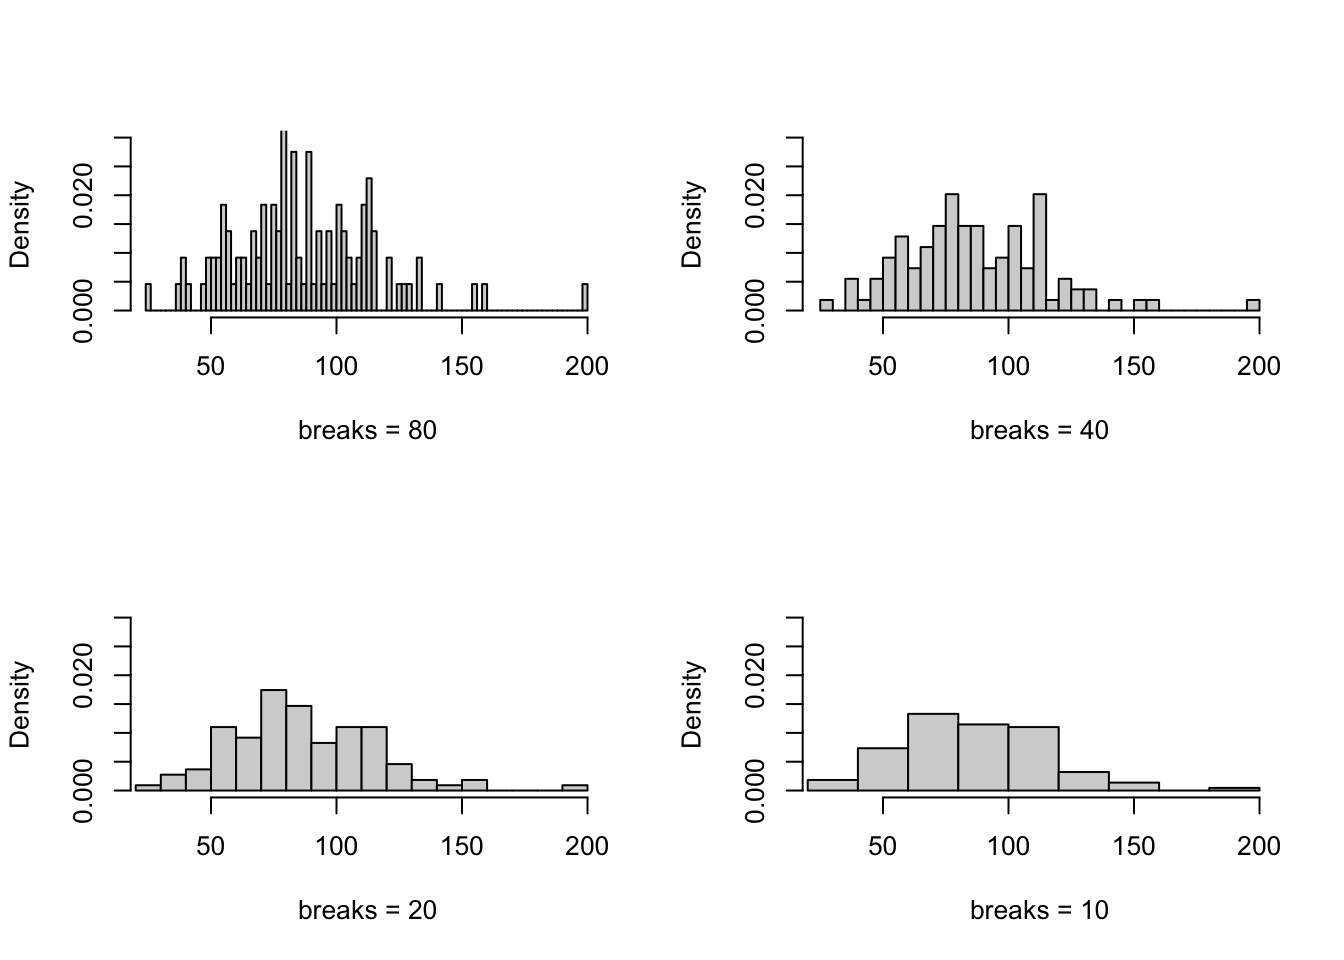
\includegraphics{MATH5714M_files/figure-latex/snow-hist-col-1.pdf}
\caption{\label{fig:snow-hist-col}This figure illustrates how the bucket size in a histogram can be controlled in R.}
\end{figure}

\hypertarget{kernel-density-estimation}{%
\subsection{Kernel Density Estimation}\label{kernel-density-estimation}}

Kernel density estimation allows to estimate the density \(f\) for given
data while avoiding some of the disadvantages of histograms.
Again, we suppose that we are given data \(x_1, \ldots, x_n \in \mathbb{R}\)
and that we want to estimate the density \(f\).

\hypertarget{motivation}{%
\subsubsection{Motivation}\label{motivation}}

Similar to the argument in the previous subsection, for \(x\) in a ``small''
interval \([a,b]\) we can estimate \(f(x)\) as
\begin{equation*}
  f(x)
  \approx \frac{1}{b-a} \int_a^b f(y) \,dy
  = \frac{1}{b-a} P\bigl( X\in [a,b] \bigr)
  \approx \frac{1}{b-a} \frac{n_{a,b}}{n},
\end{equation*}
where \(n_{a,b}\) denotes the number of samples in the interval \([a, b]\).
This equation contains two approximation. The first one,
\(f(x) \approx 1/(ba) \int_a^b f(y) \,dy\), is more accurate if the
interval is small, because then \(f\) will be nearly constant over the
interval. The second approximation will be more accurate if the
interval is large, because then the interval \([a,b]\) covers more samples
and the estimate of the probability is based on more data. We will later
discuss in detail how these two concerns can be optimally balanced.

A mathematical ``trick'' to write more clearly how \(n_{a,b}\) depends on the
data is to write the value as
\begin{equation*}
  n_{a,b}
  = \sum_{i=1}^n I_{[a,b]}(x_i),
\end{equation*}
where
\begin{equation*}
  I_{[a,b]}(x)
  = \begin{cases}
    1 & \mbox{if $x \in [a,b]$, and} \\
    0 & \mbox{otherwise.}
  \end{cases}
\end{equation*}
The function \(I_{[a,b]}\) is called the \textbf{indicator function} of the
set~\([a, b]\).

Using the indicator function notation, the estimate for \(f(x)\)
can be written as
\begin{align*}
  f(x)
  \approx \frac{1}{n(b-a)} n_{a,b}
  = \frac{1}{n} \sum_{i=1}^n \frac{1}{b-a} I_{[a,b]}(x_i)
\end{align*}
whenever \(x \in [a,b]\) and when \(b-a\) is ``not too large and not too small''.
For symmetry we choose the interval \([a, b]\) centred around \(x\),
say \([a, b] = [x - h, x + h]\) where \(h\) can be chosen to control the
width of the interval. In this case we have \(b - a = x + h - x + h = 2h\) and thus
\begin{align*}
  f(x)
  &\approx \frac{1}{n} \sum_{i=1}^n \frac{1}{2h} I_{[x-h,x+h]}(x_i) \\
  &= \frac{1}{n} \sum_{i=1}^n \frac{1}{2h} I_{[-h,+h]}(x_i-x) \\
  &= \frac{1}{n} \sum_{i=1}^n \frac{1}{2h} I_{[-1,+1]}\Bigl(\frac{x_i-x}{h}\Bigr)
\end{align*}
for all \(x \in \mathbb{R}\). This is an example of a kernel density estimate.
The function \(K(x) = 1/2 \, I_{[-1,+1]}(x)\) on the right-hand side is
called the kernel of the estimate, and the parameter \(h\) is called the
\textbf{bandwidth} or the smoothing parameter.

\hypertarget{definition-of-a-kernel-density-estimator}{%
\subsubsection{Definition of a Kernel Density Estimator}\label{definition-of-a-kernel-density-estimator}}

The general kernel density estimate is a generalisation of the idea
from the previous subsection. We first define the class of functions
which we use to replace the function \(1/2 \, I_{[-1,+1]}\).

\begin{definition}
\protect\hypertarget{def:kernel}{}\label{def:kernel}

A \textbf{kernel} is a function \(K\colon \mathbb{R}\to \mathbb{R}\) such that

\begin{itemize}
\tightlist
\item
  \(\int_{-\infty}^\infty K(x) \,dx = 1\),
\item
  \(K(x) = K(-x)\) (i.e.~\(K\) is \emph{symmetric}) and
\item
  \(K(x) \geq 0\) (i.e.~\(K\) is \emph{positive}) for all \(x\in \mathbb{R}\).
\end{itemize}

\end{definition}

Of these three properties, the first one is the most important one.
The second condition, symmetry, ensures that \(K\) is centred around \(0\)
and the third definition, positivity, makes \(K\) a probability density.
(While most authors list all three properties shown above, sometimes
the third condition is omitted.)

It is easy to check that \(K(x) = 1/2 \, I_{[-1,+1]}(x)\) satisfies all
three conditions of definition~\ref{def:kernel}. This function \(K\)
is sometimes called the ``uniform kernel'', because it is the density
of the uniform distribution~\(\mathcal{U}[-1,+1]\).

Based on the concept of a kernel, we now can define
what a Kernel Density Estimate is.

\begin{definition}
\protect\hypertarget{def:KDE}{}\label{def:KDE}For a kernel~\(K\), bandwidth~\(h > 0\) and \(x \in \mathbb{R}\), the
\textbf{kernel density estimate} for \(f(x)\) is given by
\begin{equation*}
  \hat f_h(x)
  = \frac{1}{n} \sum_{i=1}^n K_h(x - x_i),
\end{equation*}
where \(K_h\) is given by
\begin{equation*}
  K_h(y)
  = \frac{1}{h} K(y/h)
\end{equation*}
for all \(y\in \mathbb{R}\).
\end{definition}

For \(K(x) = 1/2 \, I_{[-1,+1]}(x)\) this definition recovers the
approximation we discussed in the previous section. In later sections
we will see how the kernel \(K\) can be chosen for the estimator \(\hat f\) to have ``good'' properties. As a simple example we note that if \(K\)
is continuous, then the rescaled kernel \(K_h\) and thus also the
estimate \(f_h\) are continuous functions.

Similar to the bucket width in histograms, the bandwidth parameter~\(h\)
controls how smooth the density estimate~\(\hat f_h\) is, as a function
of~\(x\).

\hypertarget{kernels}{%
\subsubsection{Kernels}\label{kernels}}

There are many different kernels in use. Some examples are listed
below. A more exhautive list can, for example, be found
\href{https://en.wikipedia.org/wiki/Kernel_(statistics)\#Kernel_functions_in_common_use}{on Wikipedia}.

\hypertarget{uniform-kernel}{%
\paragraph{Uniform Kernel}\label{uniform-kernel}}

\begin{equation*}
  K(x)
  = \begin{cases}
      1/2 & \mbox{if $-1 \leq x \leq 1$} \\
      0 & \mbox{otherwise}
    \end{cases}
\end{equation*}

\includegraphics{MATH5714M_files/figure-latex/kUniform-1.pdf}

\hypertarget{triangular-kernel}{%
\paragraph{Triangular Kernel}\label{triangular-kernel}}

\begin{equation*}
  K(x)
  = \begin{cases}
      1-|x| & \mbox{if $-1 \leq x \leq 1$} \\
      0 & \mbox{otherwise}
    \end{cases}
\end{equation*}

\includegraphics{MATH5714M_files/figure-latex/kTriangular-1.pdf}

\hypertarget{epanechnikov-kernel}{%
\paragraph{Epanechnikov Kernel}\label{epanechnikov-kernel}}

\begin{equation*}
  K(x)
  = \begin{cases}
      \frac34 (1-x^2) & \mbox{if $-1 \leq x \leq 1$} \\
      0 & \mbox{otherwise}
    \end{cases}
\end{equation*}

\includegraphics{MATH5714M_files/figure-latex/kEpanechnikov-1.pdf}

\hypertarget{gaussian-kernel}{%
\paragraph{Gaussian Kernel}\label{gaussian-kernel}}

\begin{equation*}
  K(x)
  = \frac{1}{\sqrt{2\pi}} \exp\bigl(-x^2/2\bigr)
\end{equation*}

\includegraphics{MATH5714M_files/figure-latex/kGaussian-1.pdf}

\hypertarget{kernel-density-estimation-in-r}{%
\subsection{Kernel Density Estimation in R}\label{kernel-density-estimation-in-r}}

Kernel density estimates can be computed in R using the built-in
\texttt{density()} function. If \texttt{x} is a vector containing the data, then
\texttt{density(x)} computes a basic kernel density estimate, using the
Gaussian kernel. The function has a number of optional arguments,
which can be used to control details of the estimate:

\begin{itemize}
\item
  \texttt{bw\ =\ ...} can be used to control the bandwidth~\(h\).
  If no numeric value is given, a heuristic is used.
  Note that for some kernels, \texttt{bw} differs from our \(h\)
  by a constant factor. The value \texttt{bw=1} always corresponds
  to the case where the probability distribution with density
  \(K_h\) has variance~1.
\item
  \texttt{kernel\ =\ ...} can be used to choose the kernel.
  Choices incluse \texttt{"rectangular"} (the uniform kernel), \texttt{"triangular"},
  \texttt{"epanechnikov"} and \texttt{"gaussian"}.
\end{itemize}

Details about how to call \texttt{density()} can be found by using the
\href{https://rdrr.io/r/stats/density.html}{command \texttt{help(density)}} in R.

The return value of \texttt{density} is an R object which contains information
about the kernel density estimate.

\begin{Shaded}
\begin{Highlighting}[]
\NormalTok{m }\OtherTok{\textless{}{-}} \FunctionTok{density}\NormalTok{(snowfall)}
\FunctionTok{str}\NormalTok{(m)}
\end{Highlighting}
\end{Shaded}

\begin{verbatim}
## List of 7
##  $ x        : num [1:512] -4.17 -3.72 -3.26 -2.81 -2.35 ...
##  $ y        : num [1:512] 4.32e-06 4.98e-06 5.73e-06 6.56e-06 7.48e-06 ...
##  $ bw       : num 9.72
##  $ n        : int 109
##  $ call     : language density.default(x = snowfall)
##  $ data.name: chr "snowfall"
##  $ has.na   : logi FALSE
##  - attr(*, "class")= chr "density"
\end{verbatim}

The field \texttt{\$x} and \texttt{\$y} contain the \(x\) and~\(y\) coordinates, respectively,
of points on the \(x \mapsto \hat f_h(x)\) curve, which approximates~\(f\).
The field \texttt{\$bw} shows the numeric value for the bandwidth chosen by
the heuristic. The returned object can also directly be used
as an argument to \texttt{plot()} and \texttt{lines()}, to add the graph of \(\hat f_h\)
to a plot. The commands in figure~\ref{fig:snow-dens-col} show how the
command \texttt{density()} can be used and illustrate the effect of the
bandwidth parameter.



\begin{Shaded}
\begin{Highlighting}[]
\FunctionTok{par}\NormalTok{(}\AttributeTok{mfrow =} \FunctionTok{c}\NormalTok{(}\DecValTok{2}\NormalTok{,}\DecValTok{2}\NormalTok{))}

\ControlFlowTok{for}\NormalTok{ (bw }\ControlFlowTok{in} \FunctionTok{c}\NormalTok{(}\DecValTok{1}\NormalTok{, }\DecValTok{2}\NormalTok{, }\DecValTok{4}\NormalTok{, }\DecValTok{8}\NormalTok{)) \{}
  \FunctionTok{plot}\NormalTok{(}\FunctionTok{density}\NormalTok{(snowfall, }\AttributeTok{bw =}\NormalTok{ bw, }\AttributeTok{kernel =} \StringTok{"triangular"}\NormalTok{, }\AttributeTok{n =} \DecValTok{1000}\NormalTok{),}
    \AttributeTok{xlim =} \FunctionTok{c}\NormalTok{(}\DecValTok{25}\NormalTok{,}\DecValTok{200}\NormalTok{),}
    \AttributeTok{ylim =} \FunctionTok{c}\NormalTok{(}\DecValTok{0}\NormalTok{, }\FloatTok{0.03}\NormalTok{),}
    \AttributeTok{xlab =} \FunctionTok{paste}\NormalTok{(}\StringTok{"bandwidth ="}\NormalTok{, bw),}
    \AttributeTok{main =} \ConstantTok{NA}\NormalTok{)}
\NormalTok{\}}
\end{Highlighting}
\end{Shaded}

\begin{figure}
\centering
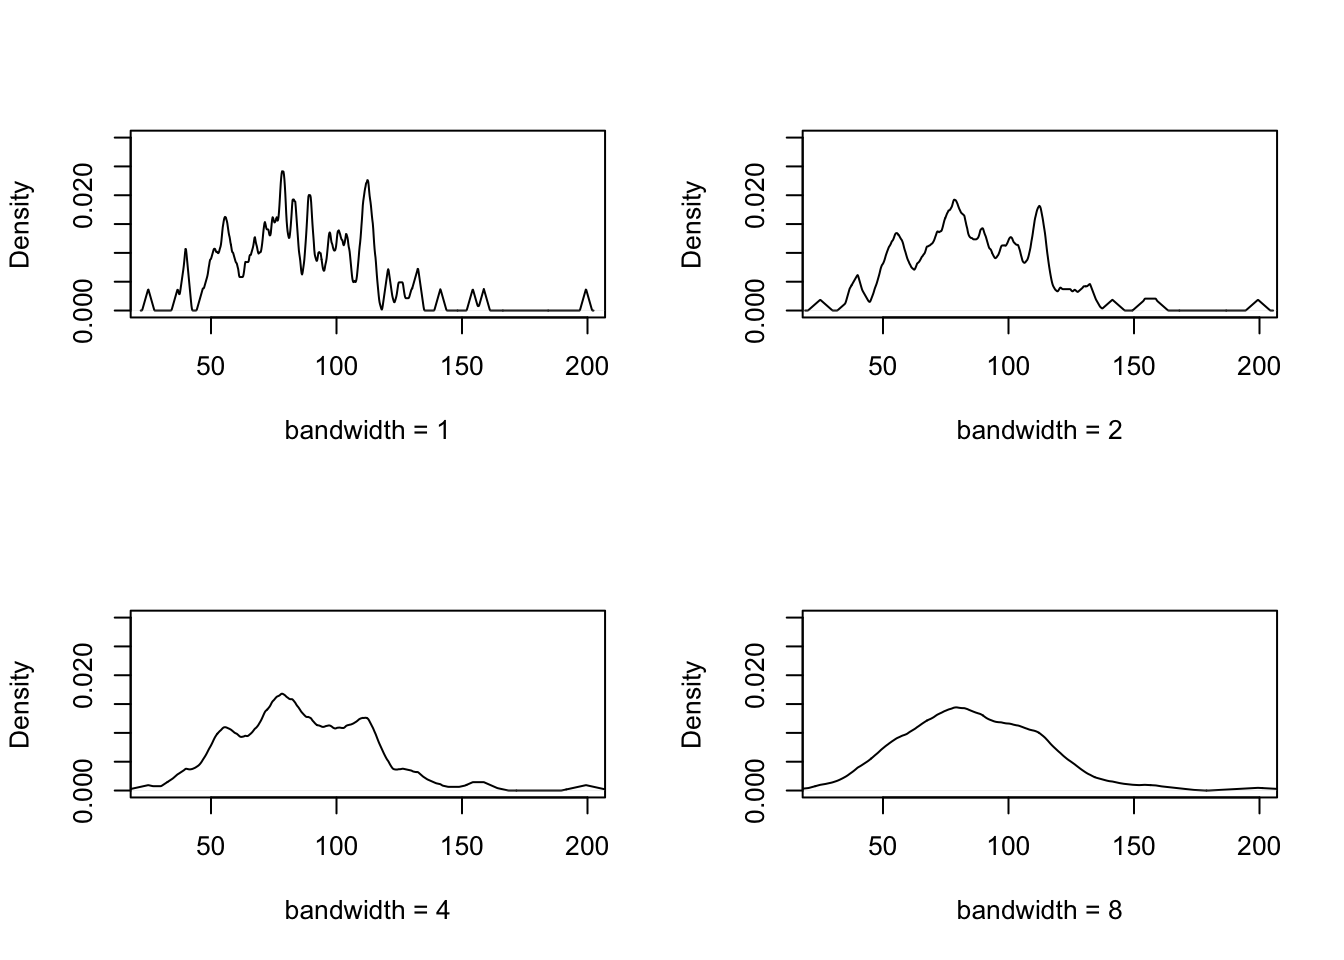
\includegraphics{MATH5714M_files/figure-latex/snow-dens-col-1.pdf}
\caption{\label{fig:snow-dens-col}This figure illustrates how the bandwidth of a kernel density estimate can be controlled in R.}
\end{figure}

\textbf{Summary}

\begin{itemize}
\tightlist
\item
  Histograms can be scaled so that they approximate densities.
\item
  Some care is needed when choosing buckets for a histogram.
\item
  Kernel density estimates can be used to estimate densities from data.
\item
  A variety of different kernel functions are commonly used.
\end{itemize}

\clearpage

\hypertarget{X02-Bias}{%
\section{The Bias of Kernel Density Estimates}\label{X02-Bias}}

In the previous section we introduced the kernel density estimate
\begin{equation}
  \hat f_h(x)
  = \frac{1}{n} \sum_{i=1}^n K_h(x - x_i)  \label{eq:KDE-est}
\end{equation}
for estimating the density \(f\), and we argued that \(\hat f_h(x) \approx f(x)\).
The aim of the current section is to quantify the error of this approximation
and to understand how this error depends on the true density~\(f\)
and on the bandwidth~\(h > 0\).

\hypertarget{a-statistical-model}{%
\subsection{A Statistical Model}\label{a-statistical-model}}

As usual, we will make a statistical model for the data \(x_1, \ldots, x_n\),
and then use this model to analyse how well the estimator performs.
The statistical model we will consider here is extremely simple: we
model the \(x_i\) using random variables
\begin{equation}
  X_1, \ldots, X_n \sim f,  \label{eq:KDE-model}
\end{equation}
which we assume to be independent and identically distributed (i.i.d.).
Here, the notation \(X \sim f\), where \(f\) is a probability density, simply
denotes that the random variable \(X\) has density~\(f\).

It is important to not confuse \(x\) (the point where we are evaluating
the densities during our analysis) with the data \(x_i\). A statistical
model describes the data, so here we get random variables \(X_1, \ldots, x_n\)
to describe the behaviour of \(x_1, \ldots, x_n\), but it does not descibe \(x\).
The number \(x\) is not part of the data, so will never be modelled by a
random variable.

While the model is very simple, for example it is much simpler than the
model we use in the level 3 part of the module for linear regression,
the associated parameter estimation problem is more challenging.
The only ``parameter'' in this model is the function \(f \colon\mathbb{R}\to \mathbb{R}\)
instead of just a vector of numbers. The space of all possible density
functions \(f\) is infinite dimensional, so this is a more challenging
estimation problem then the one we consider, for example, for linear
regression. Since \(f\) is not a ``parameter'' in the usual sense, sometimes
this problem is called a ``non-parametric'' estimation problem.

Our estimate for the density \(f\) is the function \(\hat f_h\colon \mathbb{R}\to \mathbb{R}\),
where \(\hat f_h(x)\) is given by~\eqref{eq:KDE-est} for every \(x \in\mathbb{R}\).

\hypertarget{the-bias-of-the-estimate}{%
\subsection{The Bias of the Estimate}\label{the-bias-of-the-estimate}}

As ususal, the \textbf{bias} of our estimate is the difference between
what the estimator gives on average and the truth. For our estimation
problem we get
\begin{equation*}
    \mathop{\mathrm{bias}}\bigl(\hat f_h(x)\bigr)
    = \mathbb{E}\bigl(\hat f_h(x)\bigr) - f(x).
\end{equation*}
The expectation on the right-hand side averages over the randomness
in the data, by using \(X_1, \ldots, X_n\) from the model in place of
the data.

Substituting in the definition of \(\hat f_h(x)\) from equation~\eqref{eq:KDE-est}
we find
\begin{align*}
    \mathbb{E}\bigl(\hat f_h(x)\bigr)
    &= \mathbb{E}\Bigl( \frac{1}{n} \sum_{i=1}^n K_h(x - X_i) \Bigr) \\
    &= \frac{1}{n} \sum_{i=1}^n \mathbb{E}\bigl( K_h(x - X_i) \bigr)
\end{align*}
and since the \(X_i\) are identically distributed, we can replace
all \(X_i\) with \(X_1\) (or any other of them) to get
\begin{align*}
    \mathbb{E}\bigl(\hat f_h(x)\bigr)
    &= \frac{1}{n} \sum_{i=1}^n \mathbb{E}\bigl( K_h(x - X_1) \bigr) \\
    &= \frac{1}{n} n \, \mathbb{E}\bigl( K_h(x - X_1) \bigr) \\
    &= \mathbb{E}\bigl( K_h(x - X_1) \bigr).
\end{align*}
Since the model assumes \(X_1\) (and all the other \(X_i\)) to have density~\(f\),
we can write this expectation as an integral to get
\begin{align*}
    \mathbb{E}\bigl(\hat f_h(x)\bigr)
    &= \int_{-\infty}^\infty K_h(x - y) \, f(y) \, dy \\
    &= \int_{-\infty}^\infty f(y) \, K_h(y - x) \, dy \\
    &= \int_{-\infty}^\infty f(z+x) \, K_h(z) \, dz
\end{align*}
where we used the symmetry of \(K_h\) and the substitution \(z = y - x\).

\hypertarget{moments-of-kernels}{%
\subsection{Moments of Kernels}\label{moments-of-kernels}}

To understand how the bias changes as \(h\) varies, we will need to
consider properties of \(K\) and \(K_h\) in more detail.

\begin{definition}
The \(k\)th \textbf{moment} of a kernel~\(K\),
for \(k \in \mathbb{N}_0 = \{0, 1, 2, \ldots\}\), is given by
\begin{equation*}
  \mu_k(K)
  = \int_{-\infty}^\infty x^k K(x) \,dx.
\end{equation*}
\end{definition}

The second moment \(\mu_2\) is sometimes also called the \emph{variance}
of the kernel~\(K\).

Using the properties of \(K\), we find the following results:

\begin{itemize}
\item
  Since \(x^0 = 1\) for all \(x\in\mathbb{R}\),
  the \(0\)th moment is \(\mu_0(K) = \int_{-\infty}^\infty K(x) \,dx = 1\)
  for every kernel~\(K\).
\item
  Since \(K\) is symmetric, the function \(x \mapsto x K(x)\) is
  antisymmetric and we have
  \begin{equation*}
    \mu_1(K)
    = \int_{-\infty}^\infty x K(x) \,dx
    = 0
  \end{equation*}
  for every kernel~\(K\).
\end{itemize}

The moments of the rescaled kernel \(K_h\), given by
\begin{equation*}
    K_h(x - y)
    = \frac{1}{h} K\Bigl( \frac{x-y}{h} \Bigr),
\end{equation*}
can be computed from the moments of \(K\).

\begin{lemma}
\protect\hypertarget{lem:Kh-scal}{}\label{lem:Kh-scal}Let \(K\) be a kernel, \(k \in \mathbb{N}_0\) and \(h > 0\). Then
\begin{equation*}
  \mu_k(K_h)
  = h^k \mu_k(K).
\end{equation*}
\end{lemma}

\begin{proof}
We have
\begin{align*}
  \mu_k(K_h)
  &= \int_{-\infty}^\infty x^k K_h(x) \,dx \\
  &= \int_{-\infty}^\infty x^k \frac1h K\Bigl(\frac{x}{h}\Bigr) \,dx.
\end{align*}
Using the substitution \(y = x/h\) we find
\begin{align*}
  \mu_k(K_h)
  &= \int_{-\infty}^\infty (hy)^k \frac1h K(y) \, h \,dy \\
  &= h^k \int_{-\infty}^\infty y^k K(y) \,dy \\
  &= h^k \mu_k(K).
\end{align*}
This completes the proof.
\end{proof}

It is easy to check that if \(K\) is a kernel, then \(K_h\) is also a kernel which
implies that \(K_h\) is a probability density. If \(Y\) is a random variable with
density \(K_h\), written as \(Y \sim K_h\) in short, then we find
\begin{equation*}
  \mathbb{E}(Y)
  = \int y K_h(y) \,dy
  = \mu_1(K_h)
  = 0
\end{equation*}
and
\begin{equation}
  \mathop{\mathrm{Var}}(Y)
  = \mathbb{E}(Y^2)
  = \int y^2 K_h(y) \,dy
  = \mu_2(K_h)
  = h^2 \, \mu_2(K).  \label{eq:Kh-var-Y}
\end{equation}
Thus, \(Y\) is centred and the variance of \(Y\) is proportional to~\(h^2\).

\hypertarget{the-bias-for-small-bandwidth}{%
\subsection{The Bias for Small Bandwidth}\label{the-bias-for-small-bandwidth}}

Considering again the formula
\begin{equation*}
    \mathbb{E}\bigl(\hat f_h(x)\bigr)
    = \int_{-\infty}^\infty f(x+y) \, K_h(y) \, dy,
\end{equation*}
we see that we can interpret this integral as an expectation
with respect to a random variable \(Y \sim K_h\):
\begin{equation}
    \mathbb{E}\bigl(\hat f_h(x)\bigr)
    = \mathbb{E}\bigl( f(x+Y) \bigr).  \label{eq:hf2}
\end{equation}
Equation~\eqref{eq:Kh-var-Y} shows that for \(h \downarrow 0\) the random
variable concentrates more and more around \(0\) and thus \(x+Y\) concentrates
more and more around~\(x\). For this reason we
expect~\(\mathbb{E}\bigl(\hat f_h(x)\bigr) \approx f(x)\) for small~\(h\).

To get a more qualitative version of this argument, we consider the
\href{https://en.wikipedia.org/wiki/Taylor\%27s_theorem}{Taylor approximation}
of \(f\) around the point~\(x\):
\begin{equation*}
  f(x + y)
  \approx f(x) + y f'(x) + \frac{y^2}{2} f''(x).
\end{equation*}
Substituting this into equation~\eqref{eq:hf2} we find
\begin{align*}
    \mathbb{E}\bigl(\hat f_h(x)\bigr)
    &\approx \mathbb{E}\Bigl( f(x) + Y f'(x) + \frac{Y^2}{2} f''(x) \Bigr) \\
    &= f(x) + \mathbb{E}(Y) f'(x) + \frac12 \mathbb{E}(Y^2) f''(x) \\
    &= f(x) + \frac12 h^2 \mu_2(K) f''(x)
\end{align*}
for small \(h\). Considering the bias again, this gives
\begin{equation}
  \mathop{\mathrm{bias}}\bigl( \hat f_h(x) \bigr)
  = \mathbb{E}\bigl( \hat f_h(x) \bigr) - f(x)
  \approx \frac{\mu_2(K) f''(x)}{2} h^2  \label{eq:fhatbias}
\end{equation}
which shows that the bias of the estimator descreases quadratically
as \(h\) gets smaller.

In contrast, we will see in the next section that the variance of the
estimator \emph{increases} as \(h \downarrow 0\). We will need to balance these
two effects to find the optimal value of~\(h\).

\textbf{Summary}

\begin{itemize}
\tightlist
\item
  We have introduced a statistical model for density estimation.
\item
  The bias for kernel density estimation can be written as an integral.
\item
  We learned how the moments of a kernel are defined.
\item
  The bias for small bandwidth depends on the second moment of the
  kernel and the second derivative of the density.
\end{itemize}

\clearpage

\hypertarget{X03-Var}{%
\section{The Variance of Kernel Density Estimates}\label{X03-Var}}

In the previous section we considered the bias of the estimator
\begin{equation*}
  \hat f_h(x)
  = \frac{1}{n} \sum_{i=1}^n K_h(x - x_i).
\end{equation*}
We found
\begin{equation}
  \mathbb{E}\bigl( \hat f_h(x) \bigr)
  = \mathbb{E}\bigl( K_h(x - X_i) \bigr)  \label{eq:E-hat-f-K-h}
\end{equation}
for all \(i \in \{1, \ldots, n\}\) (we used \(i=1\)), and we used this relation
to compute the bias. In this section, we will use similar arguments to compute
the variance and the mean squared error of the estimator.

\hypertarget{variance}{%
\subsection{Variance}\label{variance}}

We use the formula
\begin{equation*}
  \mathop{\mathrm{Var}}\bigl( \hat f_h(x) \bigr)
  = \mathbb{E}\bigl( \hat f_h(x)^2 \bigr) - \mathbb{E}\bigl( \hat f_h(x) \bigr)^2
\end{equation*}
and consider the two terms separately.

\hypertarget{second-moment}{%
\subsubsection{Second Moment}\label{second-moment}}

For the second moment term in the definition of the variance we get
\begin{align*}
  \mathbb{E}\bigl( \hat f_h(x)^2 \bigr)
  &= \mathbb{E}\Bigl( \frac{1}{n} \sum_{i=1}^n K_h(x - X_i) \frac{1}{n} \sum_{j=1}^n K_h(x - X_j) \Bigr) \\
  &= \frac{1}{n^2} \mathbb{E}\Bigl( \sum_{i,j=1}^n K_h(x - X_i) K_h(x - X_j) \Bigr) \\
  &= \frac{1}{n^2} \sum_{i,j=1}^n \mathbb{E}\Bigl( K_h(x - X_i) K_h(x - X_j) \Bigr)
\end{align*}
Since the \(X_i\) are independent, the values of \(i\) and \(j\) in this sum do not
matter. For the \(n\) terms where \(i=j\) we can assume that both indices equal
1, and for the \(n(n-1)\) terms where \(i\neq j\) we can assume \(i=1\) and \(j=2\),
without changing the value of the expectation. So we get
\begin{align*}
  \mathbb{E}\bigl( \hat f_h(x)^2 \bigr)
  &= \frac{1}{n^2} \Bigl( n \mathbb{E}\bigl( K_h(x - X_1)^2 ) + n(n-1) \mathbb{E}\bigl( K_h(x - X_1) K_h(x - X_2) \bigr) \Bigr) \\
  &= \frac{1}{n^2} \Bigl( n \mathbb{E}\bigl( K_h(x - X_1)^2 ) + n(n-1) \mathbb{E}\bigl( K_h(x - X_1) \bigr) \mathbb{E}\bigl( K_h(x - X_2) \bigr) \Bigr) \\
  &= \frac{1}{n^2} \Bigl( n \mathbb{E}\bigl( K_h(x - X_1)^2 ) + n(n-1) \mathbb{E}\bigl( K_h(x - X_1) \bigr)^2 \Bigr) \\
  &= \frac{1}{n} \mathbb{E}\Bigl( K_h(x - X_1)^2 \Bigr) + \frac{n-1}{n} \mathbb{E}\bigl( \hat f_h(x) \bigr)^2,
\end{align*}
where we used equation~\eqref{eq:E-hat-f-K-h} for the last term.
Using this equation, we can write the expectation as
\begin{align*}
  \mathop{\mathrm{Var}}\bigl( \hat f_h(x) \bigr)
  &= \mathbb{E}\bigl( \hat f_h(x)^2 \bigr) - \mathbb{E}\bigl( \hat f_h(x) \bigr)^2 \\
  &= \frac{1}{n} \mathbb{E}\bigl( K_h(x - X_1)^2 ) + \Bigl(\frac{n-1}{n} - 1\Bigr) \mathbb{E}\bigl( \hat f_h(x) \bigr)^2.
\end{align*}
Since \((n-1)/n - 1 = -1/n\) we get
\begin{equation}
  \mathop{\mathrm{Var}}\bigl( \hat f_h(x) \bigr)
  = \frac{1}{n} \Bigl( \mathbb{E}\bigl( K_h(x - X_1)^2 ) - \mathbb{E}\bigl( \hat f_h(x) \bigr)^2 \Bigr).
                                                          \label{eq:Var-hat-f-2}
\end{equation}

\hypertarget{the-roughness-of-a-kernel}{%
\subsubsection{The Roughness of a Kernel}\label{the-roughness-of-a-kernel}}

Similar to what we did in the last section, we will use Taylor expansion
of \(f\) around the point \(x\) to understand the behaviour of the variance
for small~\(h\). Some more care is needed here, because this time the
result also depends on the sample size~\(n\) and we will consider the joint
limit of \(n \to \infty\) and \(h\to 0\). For the first term in
equation~\eqref{eq:Var-hat-f-2} we find
\begin{align*}
  \mathbb{E}\bigl( K_h(x - X_1)^2 )
  &= \int K_h(x - y)^2 f(y) \,dy \\
  &= \int K_h(y - x)^2 f(y) \,dy \\
  &= \int \frac{1}{h^2} K\Bigl( \frac{y - x}{h} \Bigr)^2 f(y) \,dy.
\end{align*}
Now we use the substitution \(z = (y - x) / h\). This gives
\begin{align*}
  \mathbb{E}\bigl( K_h(x - X_1)^2 )
  &= \int \frac{1}{h^2} K(z)^2 f(x + hz) \,h \,dz
\end{align*}
Finally, we use Taylor approximation to get
\begin{align*}
  \mathbb{E}\bigl( K_h(x - X_1)^2 )
  &\approx \int \frac{1}{h} K(z)^2 \Bigl( f(x) + hz\,f'(x) + \frac12 h^2 z^2 \,f''(x) \Bigr) \,dz \\
  &= \frac{1}{h} f(x) \int K(z)^2 \,dz
      + f'(x) \int z K(z)^2 \,dz
      + \frac12 h f''(x) \int z^2 K(z)^2 \,dz \\
  &= \frac{1}{h} f(x) \int K(z)^2 \,dz
      + \frac12 h f''(x) \int z^2 K(z)^2 \,dz
\end{align*}
where the first-order term disappears since \(z \mapsto z K(z)^2\) is an
asymmetric function. As a shorthand we use the following definition.

\begin{definition}
The \textbf{roughness} of a kernel \(K\) is given by
\begin{equation*}
  R(K)
  := \int_{-\infty}^\infty K(x)^2 \,dx.
\end{equation*}
\end{definition}

This gives the result
\begin{equation}
  \mathbb{E}\bigl( K_h(x - X_1)^2 \bigr)
  \approx \frac{1}{h} f(x) R(K) + \frac12 h f''(x) \int z^2 K(z)^2 \,dz
                             \label{eq:Var-frag1}
\end{equation}
for small \(h\).

\hypertarget{the-variance-for-small-bandwidth}{%
\subsubsection{The Variance for Small Bandwidth}\label{the-variance-for-small-bandwidth}}

Here we consider the term \(\mathbb{E}\bigl( \hat f_h(x) \bigr)^2\) in the formula
for the variance. From the previous section we know
\begin{equation*}
    \mathbb{E}\bigl( \hat f_h(x) \bigr)
    \approx f(x) + \frac12 h^2 \mu_2(K) f''(x)
\end{equation*}
and thus we get
\begin{equation}
    \mathbb{E}\bigl( \hat f_h(x) \bigr)^2
    \approx f(x)^2 + h^2 \mu_2(K) f(x) f''(x) + \frac14 h^4 \mu_2(K)^2 f''(x)^2
                             \label{eq:Var-frag2}
\end{equation}
for small \(h\).

Substituting \eqref{eq:Var-frag1} and~\eqref{eq:Var-frag2} into
equation~\eqref{eq:Var-hat-f-2} we finally find
\begin{equation*}
  \mathop{\mathrm{Var}}\bigl( \hat f_h(x) \bigr)
  = \frac{1}{n} \Bigl(
    \frac{1}{h} f(x) R(K)
    - f(x)^2
    + \cdots
   \Bigr),
\end{equation*}
where all the omitted terms go to zero as \(h \downarrow 0\).
Omitting one more term and keeping only the leading term
we find
\begin{equation}
  \mathop{\mathrm{Var}}\bigl( \hat f_h(x) \bigr)
  \approx \frac{1}{nh} f(x) R(K)     \label{eq:fhatvar}
\end{equation}
as~\(h\downarrow 0\).

\hypertarget{mean-squared-error}{%
\subsection{Mean Squared Error}\label{mean-squared-error}}

The Mean Squared Error of the estimator \(\hat f_h(x)\) for \(f(x)\) is given
by
\begin{equation*}
  \mathop{\mathrm{MSE}}\nolimits\bigl( \hat f_h(x) \bigr)
  = \mathbb{E}\Bigl( \bigl( \hat f_h(x) - f(x) \bigr)^2 \Bigr).
\end{equation*}
It is an easy exercise to show that this can equivalently be written as
\begin{equation*}
  \mathop{\mathrm{MSE}}\nolimits\bigl( \hat f_h(x) \bigr)
  = \mathop{\mathrm{Var}}\bigl( \hat f_h(x) \bigr) + \mathop{\mathrm{bias}}\bigl( \hat f_h(x) \bigr)^2.
\end{equation*}
Substituing equations \eqref{eq:fhatbias} and~\eqref{eq:fhatvar} into
the formula for the MSE, we get
\begin{equation}
  \mathop{\mathrm{MSE}}\nolimits\bigl( \hat f_h(x) \bigr)
  \approx \frac{1}{nh} f(x) R(K) + \frac14 \mu_2(K)^2 f''(x)^2 h^4.
                           \label{eq:f-hat-MSE}
\end{equation}

Some care is needed to make sure that the omitted terms from the Taylor
approximations really don't make a significant contribution in this formula for
the MSE: The additional contributions from the variance have the form \(e_1(h) / n\), where the error term \(e_1\) does not depend on \(n\) and is negligible
compared to \(f(x) R(K) / h\) as \(h \downarrow 0\). Using
\href{https://en.wikipedia.org/wiki/Big_O_notation\#Little-o_notation}{little-o notation},
This is sometimes denoted by \(e_1(h) = o(1/h)\), which indicates that \(e_1(h) / (1/h) \to 0\) as \(h \downarrow 0\). The additional terms from the squared bias, say
\(e_2(h)\), do not depend on \(n\) and are negligible compared to \(\mu_2(K)^2 f''(x)^2 h^4\). We can write \(e_2(h) = o(h^4)\) as \(n \downarrow 0\), to reflect
this fact. We can summarise these results as
\begin{equation*}
  \mathop{\mathrm{MSE}}\nolimits\bigl( \hat f_h(x) \bigr)
  = \frac{1}{nh} f(x) R(K)
      + \frac14 \mu_2(K)^2 f''(x)^2 h^4
      + o(1/nh) + o(h^4)
\end{equation*}
as \(h \downarrow 0\),
with the understanding that the constants in the definition of \(o(h^4)\)
do not depend on \(n\) and that \(o(1/nh)\) really means ``\(o(1/h)\), where the
constants are proportional to \(1/n\).''

\hypertarget{optimal-bandwidth}{%
\subsection{Optimal Bandwidth}\label{optimal-bandwidth}}

The two terms on the right-hand side of \eqref{eq:f-hat-MSE} are balanced in
that the first term decreases for large \(h\) while the second term decreases for
small \(h\). By taking derivatives with respect to \(h\), we can
find the optimal value of \(h\). Ignoring the higher order terms, we get
\begin{equation*}
  \frac{\partial}{\partial h} \mathop{\mathrm{MSE}}\nolimits\bigl( \hat f_h(x) \bigr)
  = -\frac{1}{nh^2} f(x) R(K) + \mu_2(K)^2 f''(x)^2 h^3
\end{equation*}
and thus the derivative equals zero, if
\begin{equation*}
  \frac{1}{nh^2} f(x) R(K) = \mu_2(K)^2 f''(x)^2 h^3
\end{equation*}
or, equivalently,
\begin{equation*}
  h
  = h_\mathrm{opt}
  := \Bigl( \frac{f(x) R(K)}{n \mu_2(K)^2 f''(x)^2} \Bigr)^{1/5}.
\end{equation*}
It is easy to check that this \(h\) corresponds to the minimum of the MSE.
This shows how the optimal bandwidth depends both on the kernel and on
the target density~\(f\). In practice, this formula is hard to use,
since \(f''\) is unknown. (We don't even know \(f\)!)

Substituting the optimal value of \(h\) back into equation~\eqref{eq:f-hat-MSE},
we get
\begin{align*}
  \mathop{\mathrm{MSE}}\nolimits_\mathrm{opt}
  &= \frac{1}{n} f(x) R(K) \Bigl( \frac{n \mu_2(K)^2 f''(x)^2}{f(x) R(K)} \Bigr)^{1/5}
     + \frac14 \mu_2(K)^2 f''(x)^2 \Bigl( \frac{f(x) R(K)}{n \mu_2(K)^2 f''(x)^2} \Bigr)^{4/5} \\
  &= \frac54 \; \frac{1}{n^{4/5}}
      \; \Bigl( R(K)^2 \mu_2(K) \Bigr)^{2/5}
      \; \Bigl( f(x)^2 |f''(x)| \Bigr)^{2/5}.
\end{align*}
This expression clearly shows the contribution of \(n\), \(K\) and \(f\):

\begin{itemize}
\item
  If the bandwidth is chosen optimally, as \(n\) increases the bandwidth~\(h\)
  decreases proportionally to \(1/n^{1/5}\) and the MSE decreases
  proportionally to \(1 / n^{4/5}\). For comparison, in a Monte Carlo
  estimate for an expectation, the MSE decreases proportionally to \(1/n\).
  The error in kernel density estimation decreases slightly slower than
  for Monte Carlo estimates.
\item
  The error is proportional to \(\bigl( R(K)^2 \mu_2(K) \bigr)^{2/5}\).
  Thus we should use kernels where the value \(R(K)^2 \mu_2(K)\)
  is small.
\item
  The error is proportional to \(f(x)^2 |f''(x)|\). We cannot influence
  this term, but we can see that \(x\) where \(f\) is large or has
  high curvature have higher estimation error.
\end{itemize}

\textbf{Summary}

\begin{itemize}
\tightlist
\item
  We found the variance of the kernel density estimate.
\item
  We studied the mean squared error for small \(h\).
\item
  We derived a formula for the optimal value of the bandwidth~\(h\).
\end{itemize}

\clearpage

\hypertarget{X04-practice}{%
\section{Kernel Density Estimation in Practice}\label{X04-practice}}

In this section we conclude our discussion of kernel density estimation
by considering different aspects which are important when using the method
in practice.

\hypertarget{integrated-error}{%
\subsection{Integrated Error}\label{integrated-error}}

From equation~\eqref{eq:f-hat-MSE} we know
\begin{equation*}
  \mathop{\mathrm{MSE}}\nolimits\bigl( \hat f_h(x) \bigr)
  \approx \frac{1}{nh} f(x) R(K) + \frac14 \mu_2(K)^2 f''(x)^2 h^4.
\end{equation*}
This gives the mean squared error when trying to estimate the density
\(f(x)\) at a fixed point~\(x\). Usually we are interested in estimating
the function \(f\) rather than individual points \(f(x)\). In this case,
we consider the \textbf{integrated mean squared error (IMSE)}:
\begin{equation*}
  \mathrm{IMSE}\bigl( \hat f_h \bigr)
  := \int_{-\infty}^\infty \mathop{\mathrm{MSE}}\nolimits\bigl( \hat f_h(x) \bigr) \,dx.
\end{equation*}
Using our result from above we find
\begin{align*}
  \mathrm{IMSE}\bigl( \hat f_h \bigr)
  &\approx \int \Bigl( \frac{1}{nh} f(x) R(K) + \frac14 \mu_2(K)^2 f''(x)^2 h^4 \Bigr) \,dx \\
  &= \frac{1}{nh} R(K) \int f(x) \,dx + \frac{h^4}{4} \mu_2(K)^2 \int f''(x)^2 \,dx \\
  &= \frac{1}{nh} R(K) + \frac{1}{4} \mu_2(K)^2 R(f'') h^4,
\end{align*}
where we (mis-)use the definition of roughness as an abbreviation to express
the integral over~\(f''\).

As before, we can use differentiation to find the optimal value of \(h\).
Here we get
\begin{equation*}
  h_\mathrm{opt}
  = \Bigl( \frac{R(K)}{n \mu_2(K)^2 R(f'')} \Bigr)^{1/5}.
\end{equation*}
and the corresponding error is
\begin{equation}
  \mathrm{IMSE}_\mathrm{opt}
  = \frac54 \; \frac{1}{n^{4/5}}
      \; \Bigl( R(K)^2 \mu_2(K) \Bigr)^{2/5}
      \; R(f'')^{1/5}.  \label{eq:IMSE-opt}
\end{equation}
Thus, in order to minimise the error we still need to choose
\(h \propto n^{-1/5}\) and we should choose a kernel \(K\) which minimises
the value~\(R(K)^2 \mu_2(K)\).

\hypertarget{choice-of-kernel}{%
\subsection{Choice of Kernel}\label{choice-of-kernel}}

The integrated error in equation~\eqref{eq:IMSE-opt} is proportional to
\(\bigl( R(K)^2 \mu_2(K) \bigr)^{2/5}\), and none of the remaining terms in
the equation depends on the choice of the kernel. Thus, we can minimise
the error by choosing a kernel which has minimal \(R(K)^2 \mu_2(K)\).
For a given kernel, it is easy to work out the value of \(R(K)^2 \mu_2(K)\).

\begin{example}
For the uniform kernel we have
\begin{equation*}
  K(x)
  = \begin{cases}
      1/2 & \mbox{if $-1 \leq x \leq 1$} \\
      0 & \mbox{otherwise.}
    \end{cases}
\end{equation*}
From this we find
\begin{equation*}
  R(K)
  = \int_{-\infty}^\infty K(x)^2 \,dx
  = \int_{-1}^1 \frac14 \,dx
  = \frac12
\end{equation*}
and
\begin{equation*}
  \mu_2(K)
  = \int_{-\infty}^\infty x^2 K(x) \,dx
  = \int_{-1}^1 \frac12 x^2 \,dx
  = \frac16 \Bigl. x^3 \Bigr|_{x=-1}^1
  = \frac16 \bigl( 1 - (-1) \bigr)
  = \frac13.
\end{equation*}
Thus, for the triangular kernel we have
\begin{equation*}
  R(K)^2 \mu_2(K)
  = \Bigl( \frac12 \Bigr)^2 \frac13
  = \frac{1}{12}
  \approx 0.083333.
\end{equation*}
\end{example}

Calculations similar to the ones in the example give the following
values:

\begin{longtable}[]{@{}
  >{\raggedleft\arraybackslash}p{(\columnwidth - 8\tabcolsep) * \real{0.1300}}
  >{\centering\arraybackslash}p{(\columnwidth - 8\tabcolsep) * \real{0.5100}}
  >{\centering\arraybackslash}p{(\columnwidth - 8\tabcolsep) * \real{0.1400}}
  >{\centering\arraybackslash}p{(\columnwidth - 8\tabcolsep) * \real{0.1400}}
  >{\raggedright\arraybackslash}p{(\columnwidth - 8\tabcolsep) * \real{0.0800}}@{}}
\toprule
\begin{minipage}[b]{\linewidth}\raggedleft
kernel
\end{minipage} & \begin{minipage}[b]{\linewidth}\centering
\end{minipage} & \begin{minipage}[b]{\linewidth}\centering
\(\mu_2(K)\)
\end{minipage} & \begin{minipage}[b]{\linewidth}\centering
\(R(K)\)
\end{minipage} & \begin{minipage}[b]{\linewidth}\raggedright
\(R(K)^2 \mu_2(K)\)
\end{minipage} \\
\midrule
\endhead
Uniform & \includegraphics[width=4cm,height=\textheight]{MATH5714M_files/figure-html/kUniform-1.pdf} & \(\displaystyle\frac13\) & \(\displaystyle\frac12\) & \(0.08333\) \\
Triangular & \includegraphics[width=4cm,height=\textheight]{MATH5714M_files/figure-html/kTriangular-1.pdf} & \(\displaystyle\frac16\) & \(\displaystyle\frac23\) & \(0.07407\) \\
Epanechnikov & \includegraphics[width=4cm,height=\textheight]{MATH5714M_files/figure-html/kEpanechnikov-1.pdf} & \(\displaystyle\frac15\) & \(\displaystyle\frac35\) & \(0.07200\) \\
Gaussian & \includegraphics[width=4cm,height=\textheight]{MATH5714M_files/figure-html/kGaussian-1.pdf} & \(1\) & \(\displaystyle\frac{1}{2\sqrt{\pi}}\) & \(0.07958\) \\
\bottomrule
\end{longtable}

The best value in the table is obtained for the Epanechnikov kernel,
with \(R(K)^2 \mu_2(K) = 9/125 = 0.072\). One can show that this value
is indeed optimal amongst all kernels. Since the difference in error
for the kernels listed abive is only a few percent, any of these kernels
would be a reasonable choice.

\hypertarget{bandwidth-selection}{%
\subsection{Bandwidth Selection}\label{bandwidth-selection}}

Our formulas for the optimal bandwidth contain the terms
\(f(x)^2 |f''(x)|\) for fixed \(x\) and \(R(f'')\) for the integrated error.
Since \(f\) is unknown, neither of these quantities are available and instead
different rules of thumb are used in the literature. Here we present
one possible choice of bandwidth estimator.

Suppose that \(f\) is a normal density, with mean \(\mu\) and variance \(\sigma^2\).
Then we have
\begin{equation*}
  f(x)
  = \frac{1}{\sqrt{2\pi\sigma^2}} \exp\bigl( - (x-\mu)^2 / 2\sigma^2 \bigr).
\end{equation*}
Taking derivatives we get
\begin{equation*}
  f'(x)
  = - \frac{1}{\sqrt{2\pi\sigma^2}} \frac{x-\mu}{\sigma^2} \exp\bigl( - (x-\mu)^2 / 2\sigma^2 \bigr)
\end{equation*}
and
\begin{equation*}
  f''(x)
  = \frac{1}{\sqrt{2\pi\sigma^2}}
      \Bigl( \frac{(x-\mu)^2}{\sigma^4} - \frac{1}{\sigma^2} \Bigr)
      \exp\bigl( - (x-\mu)^2 / 2\sigma^2 \bigr)
\end{equation*}
Patiently integrating the square of this function gives
\begin{align*}
  R(f'')
  = \int_{-\infty}^\infty f''(x)^2 \,dx
  = \cdots
  = \frac{3}{8\sigma^5\sqrt{\pi}}.
\end{align*}
This can be used as a simple ``plug-in rule'' with \(\sigma\) estimated by the
sample standard deviation.

We now demonstrate how this rule of thumb could be used in R to obtain a kernel
density estimate for the snowfall data. We will use the Epanechnikov kernel.
For compatibility with the kernels built into R, we rescale this kernel, so
that \(\mu_2(K) = 1\), i.e.~we consider \(K_{\sqrt{5}}\) in place of \(K\). An easy
calculation shows that the roughness is then \(R(K) = 3 / (5*\sqrt(5))\).

\begin{Shaded}
\begin{Highlighting}[]
\CommentTok{\# downloaded from https://teaching.seehuhn.de/data/buffalo/}
\NormalTok{x }\OtherTok{\textless{}{-}} \FunctionTok{read.csv}\NormalTok{(}\StringTok{"data/buffalo.csv"}\NormalTok{)}
\NormalTok{snowfall }\OtherTok{\textless{}{-}}\NormalTok{ x}\SpecialCharTok{$}\NormalTok{snowfall}
\NormalTok{n }\OtherTok{\textless{}{-}} \FunctionTok{length}\NormalTok{(snowfall)}

\CommentTok{\# Roughness of the Epanechnikov kernel, after rescaling with h = sqrt(5)}
\CommentTok{\# so that the second moment becomes mu\_2 = 1:}
\NormalTok{R.K }\OtherTok{\textless{}{-}} \DecValTok{3} \SpecialCharTok{/}\NormalTok{ (}\DecValTok{5} \SpecialCharTok{*} \FunctionTok{sqrt}\NormalTok{(}\DecValTok{5}\NormalTok{))}

\CommentTok{\# Rule of thumb:}
\NormalTok{R.fpp }\OtherTok{\textless{}{-}} \DecValTok{3} \SpecialCharTok{/}\NormalTok{ (}\DecValTok{8} \SpecialCharTok{*} \FunctionTok{sd}\NormalTok{(snowfall)}\SpecialCharTok{\^{}}\DecValTok{5} \SpecialCharTok{*} \FunctionTok{sqrt}\NormalTok{(pi))}

\CommentTok{\# formula for the optimal h}
\NormalTok{my.bw }\OtherTok{\textless{}{-}}\NormalTok{ (R.K }\SpecialCharTok{/}\NormalTok{ (n }\SpecialCharTok{*} \DecValTok{1}\SpecialCharTok{\^{}}\DecValTok{2} \SpecialCharTok{*}\NormalTok{ R.fpp))}\SpecialCharTok{\^{}}\FloatTok{0.2}
\NormalTok{my.bw}
\end{Highlighting}
\end{Shaded}

\begin{verbatim}
## [1] 11.58548
\end{verbatim}

R has a variety of different builtin methods to estimate bandwidths.
See stats/bandwidth for a description. For comparison to our result,
we list here the bandwidths suggested by some of R's algorithms:

\begin{Shaded}
\begin{Highlighting}[]
\FunctionTok{data.frame}\NormalTok{(}
  \AttributeTok{name =} \FunctionTok{c}\NormalTok{(}\StringTok{"nrd0"}\NormalTok{, }\StringTok{"nrd"}\NormalTok{, }\StringTok{"SJ"}\NormalTok{),}
  \AttributeTok{bw =} \FunctionTok{c}\NormalTok{(}\FunctionTok{bw.nrd0}\NormalTok{(snowfall), }\FunctionTok{bw.nrd}\NormalTok{(snowfall), }\FunctionTok{bw.SJ}\NormalTok{(snowfall)))}
\end{Highlighting}
\end{Shaded}

\begin{verbatim}
##   name        bw
## 1 nrd0  9.724206
## 2  nrd 11.452953
## 3   SJ 11.903840
\end{verbatim}

All of these value seem close the value we obtained manually. Using
our bandwidth estimate, we get the following estimated density.

\begin{Shaded}
\begin{Highlighting}[]
\FunctionTok{plot}\NormalTok{(}\FunctionTok{density}\NormalTok{(snowfall, }\AttributeTok{bw =}\NormalTok{ my.bw, }\AttributeTok{kernel =} \StringTok{"epanechnikov"}\NormalTok{),}
     \AttributeTok{main =} \ConstantTok{NA}\NormalTok{)}
\end{Highlighting}
\end{Shaded}

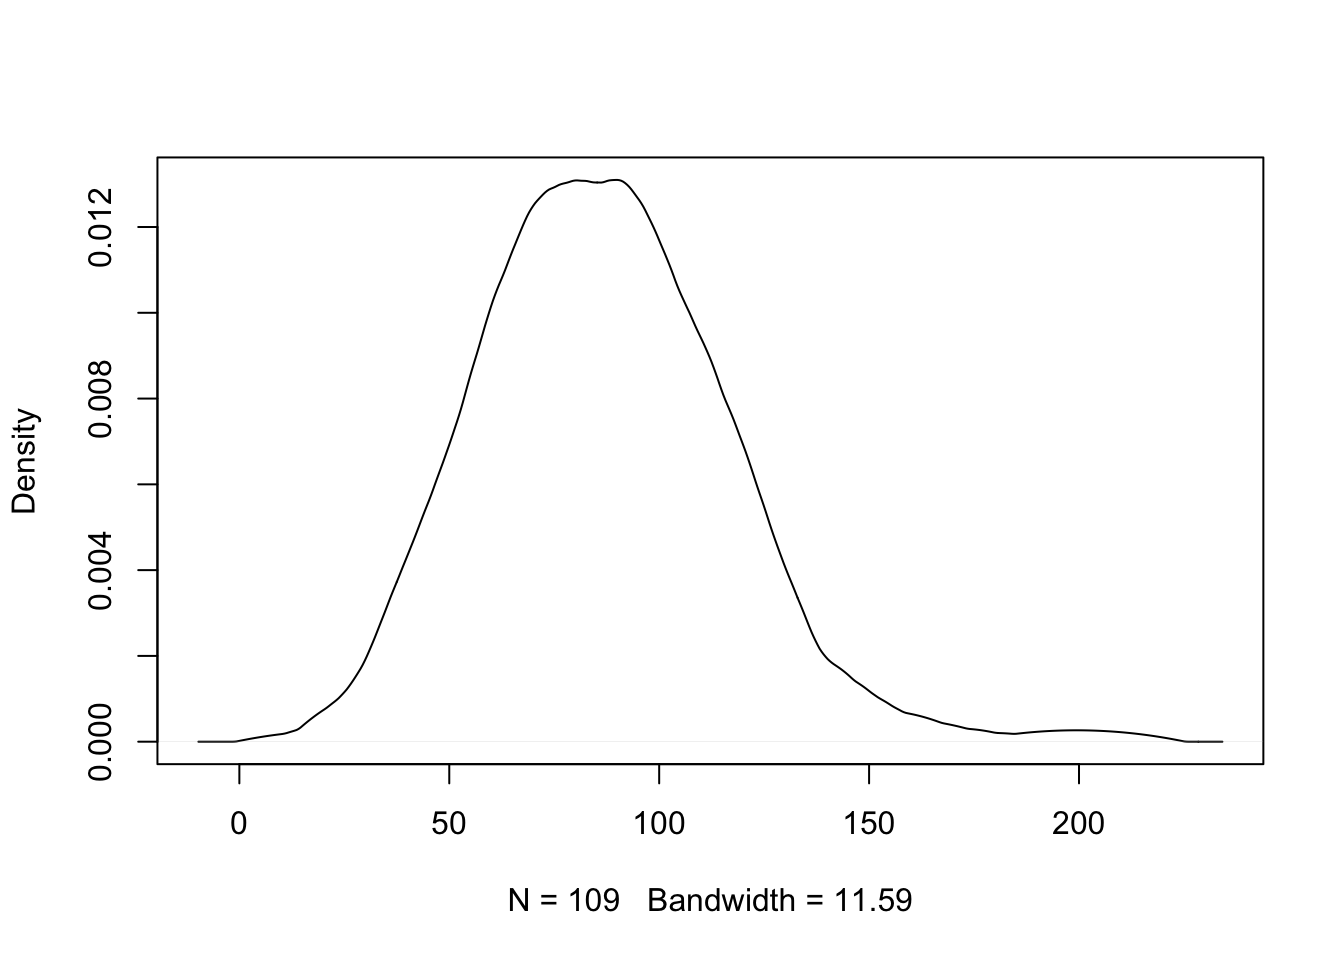
\includegraphics{MATH5714M_files/figure-latex/buffalo-final-1.pdf}

In practice one would just use one of the built-in methods, for example using
\texttt{bw="SJ"} instead of estimating the bandwidth manually.

\hypertarget{higher-dimensions}{%
\subsection{Higher Dimensions}\label{higher-dimensions}}

So far we have only considered the one-dimensional case, where the samples \(x_i\)
are real numbers. In this subsection we will sketch how these methods will need
to be adjusted for the multivariate case of \(x_i = (x_{i,1}, \ldots, x_{i,p}) \in \mathbb{R}^p\).

In this setup, a \textbf{kernel} is a function \(K\colon \mathbb{R}^p\to \mathbb{R}\) such that

\begin{itemize}
\tightlist
\item
  \(\int \cdots \int K(x) \,dx_p \cdots dx_1 = 1\),
\item
  \(K(x) = K(-x)\) and
\item
  \(K(x) \geq 0\) for all \(x\in \mathbb{R}\),
\end{itemize}

where the integral in the first condition is now over all \(p\) coordinates.

\begin{example}
If \(K_1, \ldots, K_p\) are one-dimensional kernels, then the product
\begin{equation*}
  K(x_1, \ldots, x_p)
  := K_1(x_1) \cdots K_p(x_p)
\end{equation*}
is a kernel in \(p\) dimensions. If we use the product of \(p\)
Gaussian kernels, we get
\begin{align*}
  K(x)
  &= \prod_{i=1}^p \frac{1}{\sqrt{2\pi}} \exp\bigl(-x_i^2/2\bigr) \\
  &=  \frac{1}{(2\pi)^{p/2}} \exp\Bigl(-\frac12 (x_1^2 + \cdots + x_p^2) \Bigr).
\end{align*}
\end{example}

There are different possibilities for rescaling these kernels:

\begin{itemize}
\item
  If all coordinates live on ``comparable scales'' (e.g., if they are
  measured in the same units), the formula
  \[ K_h(x) = \frac{1}{h^p} K(x/h) \]
  for all \(x\in\mathbb{R}^p\) can be used, where \(h>0\) is a bandwidth parameter
  as before. The scaling by \(1/h^p\) is required
  to ensure that the integral of \(K_h\) equals \(1\), so that \(K_h\) is
  a kernel again.
\item
  If different scaling is desirable for different components, the formula
  \begin{equation*}
    K_h(x)
    = \frac{1}{h_1 \cdots h_p} K(x_1/h_1, \ldots, x_p/h_p)
  \end{equation*}
  for all \(x\in\mathbb{R}^p\) can be used, where \(h = (h_1, \ldots, h_p)\) is a vector
  of bandwidth parameters.
\item
  A more general version would be to use a symmetric, positive definite
  bandwidth matrix \(H \in \mathbb{R}^{p\times p}\).
  In this case the required scaling is
  \begin{equation*}
    K_H(x)
    = \frac{1}{\mathrm{det}(H)} K\bigl( H^{-1} x \bigr)
  \end{equation*}
  for all \(x\in\mathbb{R}^p\).
\end{itemize}

For all of these choices, the kernel density estimator is given by
\begin{equation*}
  \hat f_h(x)
  = \frac{1}{n} \sum_{i=1}^n K_h(x - x_i)
\end{equation*}
(using \(K_H\) for the third option) for all \(x\in\mathbb{R}^p\).
Bandwidth selection in the multivariate case is a difficult problem
and we will not discuss this here.

\clearpage

\hypertarget{X05-smoothing}{%
\section{Kernel Smoothing}\label{X05-smoothing}}

We now consider the statistical model
\begin{equation*}
  Y_i
  = m(x_i) + \varepsilon_i,
\end{equation*}
where \(m\colon \mathbb{R}\to \mathbb{R}\) is a smooth function and \(\varepsilon_i\) are independent
random variables with \(\mathbb{E}(\varepsilon_i) = 0\). We are given data \((x_i, y_i)\) for
\(i\in \{1, \ldots, n\}\) and our aim is to estimate the function~\(m\). The
task of estimating the function~\(m\) from data is called \textbf{smoothing}.

\hypertarget{the-nadaraya-watson-estimator}{%
\subsection{The Nadaraya-Watson Estimator}\label{the-nadaraya-watson-estimator}}

Since we have
\begin{equation*}
  \mathbb{E}(Y_i)
  = \mathbb{E}\bigl( m(x_i) + \varepsilon_i \bigr)
  = m(x_i) + \mathbb{E}( \varepsilon_i )
  = m(x_i),
\end{equation*}
we could attempt to use a Monte-Carlo approach where we estimate the
expectation \(\mathbb{E}(Y_i)\) using an average of many \(Y\) values. This approach is
not feasible in practice, since typically we will only have \emph{a single}
observation \(y_i\) corresponding to a given \(x_i\). The idea of the
Nadaraya-Watson Estimator is to average the \(y_i\) corresponding to nearby \(x_i\)
instead. A weighted average is used, which gives less weight to further away
values. This leads to the following definition.

\begin{definition}
\protect\hypertarget{def:NW}{}\label{def:NW}The \textbf{Nadaraya-Watson Estimator} for \(m(x)\) is given by
\begin{equation*}
  \hat m_h(x)
  = \frac{\sum_{i=1}^n K_h(x - x_i) y_i}{\sum_{j=1}^n K_h(x - x_j)},
\end{equation*}
where \(K_h\) is a kernel scaled to bandwidth~\(h\) as in
definition~\ref{def:KDE}.
\end{definition}

The proble of finding \(m\) using kernel functions are called \textbf{kernel smoothing}
or \textbf{kernel regression}. In this context, the bandwidth \(h\) is also called
the \textbf{smoothing parameter}. The Nadaraya-Watson Estimator is not the only
method for kernel smoothing. We will learn about different methods in the
next sections.

Using the shorthand
\begin{equation*}
  w_i(x)
  := \frac{K_h(x - x_i)}{\sum_{j=1}^n K_h(x - x_j)}
\end{equation*}
we can write the Nadaraya-Watson Estimator as
\(\hat m_h(x) = \sum_{i=1}^n w_i(x) y_i\) and since
\begin{align*}
  \sum_{i=1}^n w_i(x)
  &= \sum_{i=1}^n \frac{K_h(x - x_i)}{\sum_{j=1}^n K_h(x - x_j)} \\
  &= \frac{\sum_{i=1}^n K_h(x - x_i)}{\sum_{j=1}^n K_h(x - x_j)} \\
  &= 1,
\end{align*}
this is indeed a weighted average.

\begin{example}
The \texttt{faithful} dataset built into R contains 272 observations of
waiting time between eruptions and the duration of the eruption for the Old Faithful geyser in Yellowstone National Park. We can use the
\texttt{ksmooth()} function to compute Nadaraya-Watson estimate for the
waiting time after an eruption of a given length. Here we use
a Gaussian kernel with bandwidth~1.

\begin{Shaded}
\begin{Highlighting}[]
\NormalTok{x }\OtherTok{\textless{}{-}}\NormalTok{ faithful}\SpecialCharTok{$}\NormalTok{eruptions}
\NormalTok{y }\OtherTok{\textless{}{-}}\NormalTok{ faithful}\SpecialCharTok{$}\NormalTok{waiting}
\FunctionTok{plot}\NormalTok{(x, y, }\AttributeTok{cex =}\NormalTok{ .}\DecValTok{5}\NormalTok{,}
     \AttributeTok{xlab =} \StringTok{"eruption time [mins]"}\NormalTok{, }\AttributeTok{ylab =} \StringTok{"time to next eruption [mins]"}\NormalTok{)}
\FunctionTok{lines}\NormalTok{(}\FunctionTok{ksmooth}\NormalTok{(x, y, }\AttributeTok{kernel =} \StringTok{"normal"}\NormalTok{, }\AttributeTok{bandwidth =} \DecValTok{1}\NormalTok{, }\AttributeTok{n.points =} \DecValTok{1000}\NormalTok{),}
      \AttributeTok{col =} \StringTok{"red"}\NormalTok{)}
\end{Highlighting}
\end{Shaded}

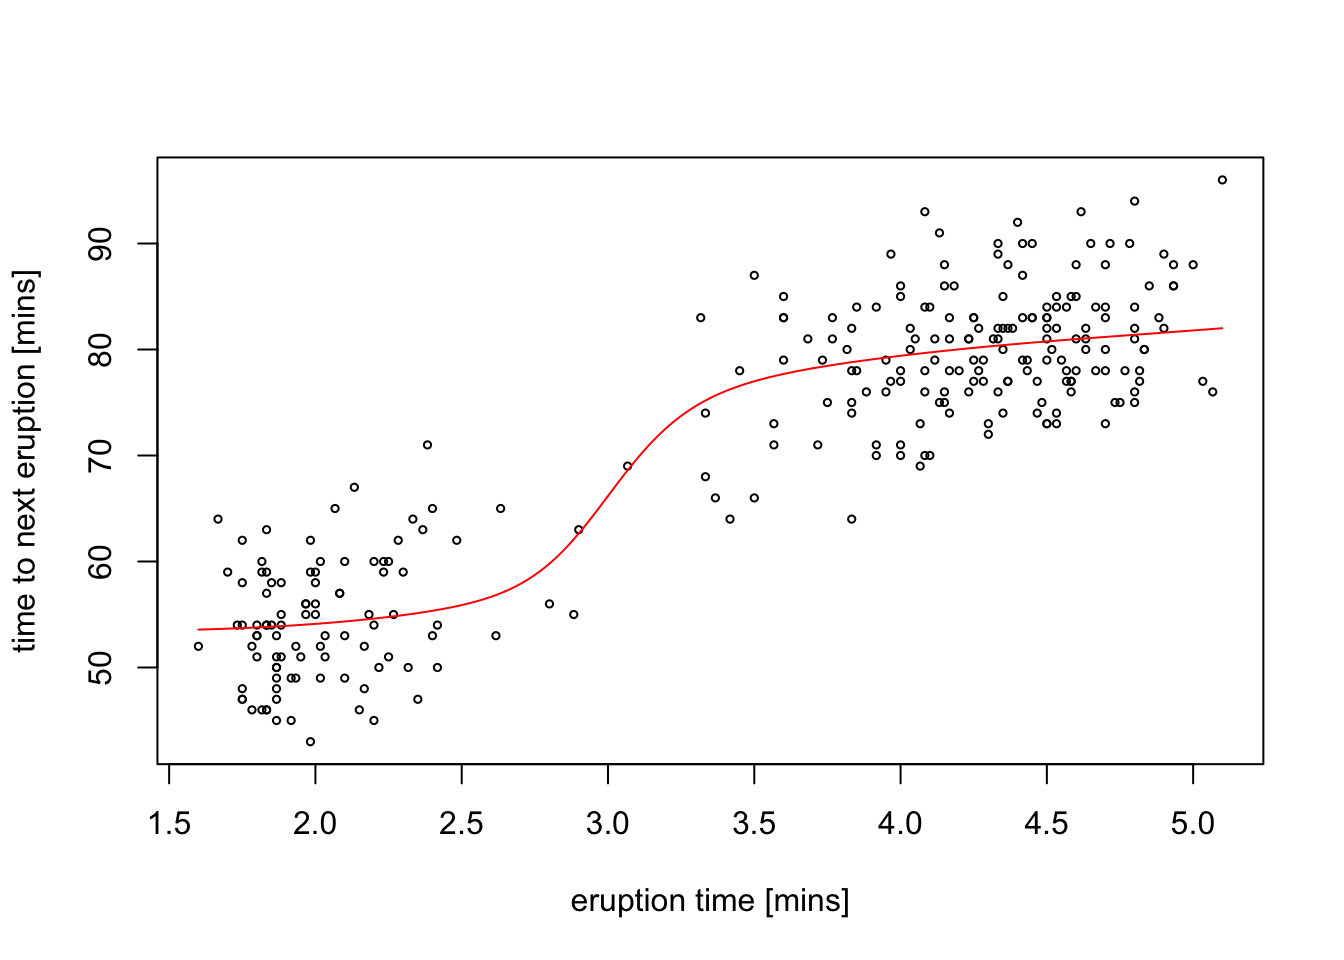
\includegraphics{MATH5714M_files/figure-latex/faithful2-1.pdf}

The estimate \(\hat m_h\) (red line) smoothly connects the two clusters
visible in the scatter plot.
\end{example}

For kernels with bounded support, \emph{e.g.}~for the Epanechnikov kernel,
the denominator \(\sum_{j=1}^n K_h(x - x_j)\) will equal zero for \(x\)
which are too far away from all of the \(x_i\). For these \(x\), the weights
\(w_i\) and thus also the estimate \(\hat m_h(x)\) are undefined. This
problem can easily be seen in practice, when the bandwidth is chosen
too small.

\begin{example}
To illustrate the problem of the estimate becoming undefined far away
from the data points, we redo the previous estimate using a uniform
kernel:

\begin{Shaded}
\begin{Highlighting}[]
\FunctionTok{plot}\NormalTok{(x, y, }\AttributeTok{cex =}\NormalTok{ .}\DecValTok{5}\NormalTok{,}
     \AttributeTok{xlab =} \StringTok{"eruption time [mins]"}\NormalTok{, }\AttributeTok{ylab =} \StringTok{"time to next eruption [mins]"}\NormalTok{)}
\FunctionTok{lines}\NormalTok{(}\FunctionTok{ksmooth}\NormalTok{(x, y, }\AttributeTok{kernel =} \StringTok{"box"}\NormalTok{, }\AttributeTok{bandwidth =} \DecValTok{1}\NormalTok{, }\AttributeTok{n.points =} \DecValTok{1000}\NormalTok{),}
      \AttributeTok{col =} \StringTok{"red"}\NormalTok{)}
\FunctionTok{lines}\NormalTok{(}\FunctionTok{ksmooth}\NormalTok{(x, y, }\AttributeTok{kernel =} \StringTok{"box"}\NormalTok{, }\AttributeTok{bandwidth =} \FloatTok{0.1}\NormalTok{, }\AttributeTok{n.points =} \DecValTok{1000}\NormalTok{),}
      \AttributeTok{col =} \StringTok{"blue"}\NormalTok{)}
\end{Highlighting}
\end{Shaded}

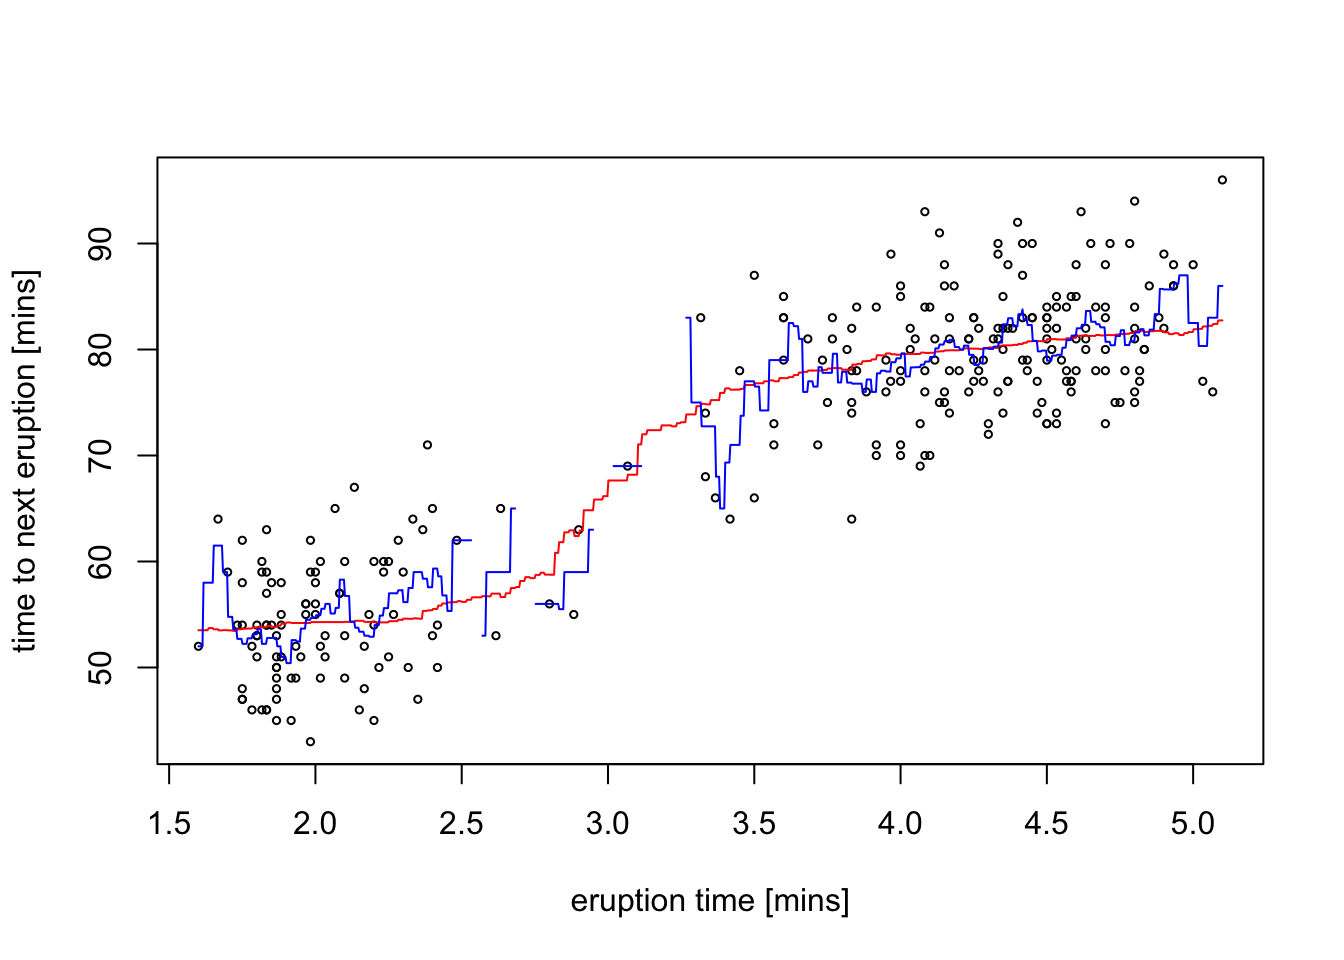
\includegraphics{MATH5714M_files/figure-latex/faithful1-1.pdf}

For \(h = 1\) (red line) we get a line \(\hat m_h\) which is less smooth than
the estimate using the Gaussian kernel, but is otherwise looks similar to
the previous estimate. In contrast, if we reduce the bandwidth to \(h = 0.1\)
(blue line), gaps start to appear in the plot of \(\hat m_h\) where the
spacing of the data points is too large.
\end{example}

\hypertarget{estimation-error}{%
\subsection{Estimation Error}\label{estimation-error}}

Here we will discuss how fast the estimation error decreases in the
limit of \(n\to \infty\), \emph{i.e.}~for the case when we have a large dateset
to use for the estimate. As before, we will find that we need to decrease
the bandwidth \(h\) as \(n\) increases.

To allow for \(n\) to change, we will introduce a statistical model
also for the inputs \(x_i\). (This is different from what we did
in the level 3 part of the module for linear regression.) Here
we will consider the following model:

\begin{itemize}
\tightlist
\item
  \(X_1, \ldots, X_n\) are independent and identically distributed with
  density~\(f\).
\item
  \(\eta_1, \ldots \eta_n\) are independent, with \(\mathbb{E}(\eta_i) = 0\)
  and \(\mathop{\mathrm{Var}}(\eta_i) = 1\).
\item
  \(\varepsilon_i = s(X_i) \eta_i\) for all \(i \in \{1, \ldots, n\}\),
  where \(s\colon \mathbb{R}\to (0, \infty)\) is a smooth function.
\item
  \(Y_i = m(X_i) + \varepsilon_i\) where \(m\colon \mathbb{R}\to \mathbb{R}\) is a smooth function.
\end{itemize}

While this extended model allows us to increase \(n\), it also creates
a practical problem: the estimator
\begin{equation*}
  \hat m_h(x)
  = \frac{\sum_{i=1}^n K_h(x - X_i) Y_i}{\sum_{j=1}^n K_h(x - X_j)},
\end{equation*}
now has random terms both in the numerator and in the denominator.
This will make it more challenging to determine the behaviour
of \(\mathbb{E}\bigl( \hat m_h(x) \bigr)\) and \(\mathop{\mathrm{Var}}\bigl( \hat m_h(x) \bigr)\)
as \(n \to \infty\) and \(h \downarrow 0\). We can write \(\hat m_h(x)\) as
\begin{equation}
  \hat m_h(x)
  = \frac{\frac1n \sum_{i=1}^n K_h(x - X_i) Y_i}{\frac1n \sum_{j=1}^n K_h(x - X_j)}
  = \frac{\frac1n \sum_{i=1}^n K_h(x - X_i) Y_i}{\hat f_h(x)}
  = \frac{\hat r_h(x)}{\hat f_h(x)}  \label{eq:m-hat-h}
\end{equation}
where \(\hat f_h(x)\) is the kernel density estimator from
\protect\hyperlink{X01-KDE}{Section 1} and
\begin{equation*}
  \hat r_h(x)
  := \frac1n \sum_{i=1}^n K_h(x - X_i) Y_i.
\end{equation*}
We will consider the numerator and denominator of equation \eqref{eq:m-hat-h}
separately

\hypertarget{denominator}{%
\subsubsection*{Denominator}\label{denominator}}
\addcontentsline{toc}{subsubsection}{Denominator}

From equations \eqref{eq:fhatbias} and \eqref{eq:fhatvar} we know that
\begin{equation*}
  \mathbb{E}\bigl( \hat f_h(x) \bigr)
  \approx f(x) + \frac{\mu_2(K) f''(x)}{2} h^2
\end{equation*}
and
\begin{equation*}
  \mathop{\mathrm{Var}}\bigl( \hat f_h(x) \bigr)
  \approx \frac{1}{nh} f(x) R(K)
\end{equation*}
as \(h \downarrow 0\).

\hypertarget{numerator}{%
\subsubsection*{Numerator}\label{numerator}}
\addcontentsline{toc}{subsubsection}{Numerator}

We start by considering the numerator \(\hat r_h(x)\). The arguments used here
will be very similar to the arguments used in the section about the
\protect\hyperlink{X03-Var}{variance of kernel density estimates}.

The expectation of \(\hat r_h(x)\) is
\begin{align*}
  \mathbb{E}\bigl( \hat r_h(x) \bigr)
  &= \mathbb{E}\Bigl( \frac1n \sum_{i=1}^n K_h(x - X_i) Y_i \Bigr) \\
  &= \frac1n \sum_{i=1}^n \mathbb{E}\bigl( K_h(x - X_i) Y_i \bigr) \\
  &= \mathbb{E}\bigl( K_h(x - X) Y \bigr) \\
  &= \mathbb{E}\Bigl( K_h(x - X) (m(X) + \sigma(X)\eta) \Bigr).
\end{align*}
We use integrals to average over the randomness in \(X\) and \(\eta\),
denoting the density of \(\eta\) by~\(\varphi\):
\begin{align*}
  \mathbb{E}\bigl( \hat r_h(x) \bigr)
  &= \int \int K_h(x - \xi) \bigl( m(\xi) + \sigma(\xi) e \bigr) \, \varphi(e) \, de \, f(\xi) \, d\xi \\
  &= \int K_h(x - \xi) \Bigl( m(\xi) +\sigma(\xi) \int e \, \varphi(e) \, de \Bigr) \, f(\xi) \, d\xi \\
  &= \int K_h(x - \xi) m(\xi) f(\xi) \, d\xi,
\end{align*}
since
\begin{equation*}
  \int e \, \varphi(e) \, de
  = \mathbb{E}(\eta)
  = 0.
\end{equation*}
Writing
\begin{equation*}
  r(x)
  := m(x) f(x)
\end{equation*}
as an abbreviation, we finally get
\begin{equation*}
  \mathbb{E}\bigl( \hat r_h(x) \bigr)
  = \int K_h(x - \xi) r(\xi) \, d\xi.
\end{equation*}

We now formalise an argument which we already used earlier.

\begin{lemma}
\protect\hypertarget{lem:kernel-limit}{}\label{lem:kernel-limit}

Let \(g\colon \mathbb{R}\to \mathbb{R}\) be two times continuously differentiable
and let \(K\) be a kernel function. Then we have

\begin{enumerate}
\def\labelenumi{\arabic{enumi}.}
\tightlist
\item
  \(\displaystyle\int K_h(x - \xi) g(\xi) \, d\xi = g(x) + \frac12 \mu_2(K) g''(x) h^2 + o(h^2)\)
  as \(h \downarrow 0\), and
\item
  \(\displaystyle\int K_h(x - \xi)^2 g(\xi) \, d\xi = \frac1h R(K) g(x) + o(1/h)\)
  as \(h \downarrow 0\).
\end{enumerate}

\end{lemma}

\begin{proof}
The first statement is proved using substitution and Taylor expandion of \(r\)
around \(x\) as shown in the derivation of equation~\eqref{eq:fhatbias}.
The second statement is proved similarly, as shown in the derivation of
equation~\eqref{eq:Var-frag1}.
\end{proof}

Using the first part of lemma~\ref{lem:kernel-limit} for \(g = r\) we get
\begin{equation*}
  \mathbb{E}\bigl( \hat r_h(x) \bigr)
  = r(x) + \frac12 \mu_2(K) r''(x) h^2 + o(h^2).
\end{equation*}

For the variance of \(\hat r_h(x)\) we get
\begin{align*}
  \mathop{\mathrm{Var}}\bigl( \hat r_h(x) \bigr)
  &= \mathop{\mathrm{Var}}\Bigl( \frac1n \sum_{i=1}^n K_h(x - X_i) Y_i \Bigr) \\
  &= \frac{1}{n^2} \sum_{i=1}^n \mathop{\mathrm{Var}}\bigl( K_h(x - X_i) Y_i \bigr) \\
  &= \frac1n \mathop{\mathrm{Var}}\bigl( K_h(x - X) Y \bigr) \\
  &= \frac1n \Bigl( \mathbb{E}\bigl( K_h(x - X)^2 Y^2 \bigr) - \mathbb{E}\bigl( K_h(x - X) Y \bigr)^2 \Bigr).
\end{align*}
We have already seen that
\begin{equation*}
  \mathbb{E}\bigl( K_h(x - X) Y \bigr)
  = \mathbb{E}\bigl( \hat r_h(x) \bigr)
  = r(x) + \frac12 \mu_2(K) r''(x) h^2 + o(h^2)
\end{equation*}
and thus
\begin{equation*}
  \mathbb{E}\bigl( K_h(x - X) Y \bigr)^2
  = r(x)^2 + O(h^2).
\end{equation*}
Using the second part of lemma~\ref{lem:kernel-limit} one can show that
\begin{align*}
  \mathbb{E}\bigl( K_h(x - X)^2 Y^2 \bigr)
  &= \int \int K_h(x - \xi)^2 \bigl( m(\xi) + s(\xi)e \bigr)^2 \,\varphi(e)\,de \,f(\xi)\,d\xi \\
  &= \int K_h(x - \xi)^2 \bigl( m(\xi)^2 + s(\xi)^2 \bigr) f(\xi) \,d\xi \\
  &= \frac1h R(K) \bigl( m(x)^2 + s(x)^2 \bigr) f(x) + o(1/h).
\end{align*}
Combining these equations we find
\begin{equation*}
  \mathop{\mathrm{Var}}\bigl( \hat r_h(x) \bigr)
  \approx \frac{1}{nh} R(K) \bigl( m(x)^2 + s(x)^2 \bigr) f(x)
    + \frac1n r(x)^2
\end{equation*}
as \(n\to\infty\), \(h\downarrow 0\) and \(nh\to\infty\).

\hypertarget{mean-squared-error-1}{%
\subsubsection*{Mean Squared Error}\label{mean-squared-error-1}}
\addcontentsline{toc}{subsubsection}{Mean Squared Error}

To turn our results about \(\hat r_h\) and our previous results about
\(\hat f\) into an error estimate for
\begin{equation*}
  \hat m_h(x)
  = \frac{\hat r_h(x)}{\hat f_h(x)},
\end{equation*}
we consider Taylor expansion of the function \(g(y) = 1/y\):
\begin{align*}
  g(y + h)
  &= g(y) + g'(y) h + o(h) \\
  &= \frac1y - \frac{1}{y^2} h + o(h).
\end{align*}
Using this approximation we get
\begin{align*}
  \hat m_h(x)
  &= \hat r_h(x) g\bigl( \hat f_h(x) \bigr) \\
  &= \hat r_h(x) g\bigl( f(x) + \hat f_h(x) - f(x) \bigr) \\
  &\approx \hat r_h(x) \Bigl( \frac{1}{f(x)} - \frac{1}{f(x)^2} (\hat f_h(x) - f(x)) \Bigr) \\
  &= \frac{\hat r_h(x)}{f(x)} - \frac{\hat r_h(x) \bigl(\hat f_h(x) - f(x) \bigr)}{f(x)^2}.
\end{align*}
With the help of this trick, we have achieved that now all random terms
are in the denominator and thus we can take expectations easily:
\begin{align*}
  \mathbb{E}\bigl( \hat m_h(x) \bigr)
  &= \frac{\mathbb{E}\bigl( \hat r_h(x) \bigr)}{f(x)}
      - \frac{\mathbb{E}\Bigl( \hat r_h(x) \bigl(\hat f_h(x) - f(x) \bigr) \Bigr)}{f(x)^2} \\
  &\approx \frac{\mathbb{E}\bigl( \hat r_h(x) \bigr)}{f(x)}
      - \frac{\mathbb{E}\bigl( \hat r_h(x) \bigr) \mathbb{E}\bigl( \hat f_h(x) - f(x) \bigr)}{f(x)^2}.
\end{align*}
Substituting in our previous results we get
\begin{align*}
  \mathbb{E}\bigl( \hat m_h(x) \bigr)
  &\approx \frac{r(x) + \frac12 \mu_2(K) r''(x) h^2 + o(h^2)}{f(x)}
      - \frac{\bigl( r(x) + \frac12 \mu_2(K) r''(x) h^2 + o(h^2) \bigr)
          \frac12 \mu_2(K) f''(x) h^2}{f(x)^2} \\
  &= \frac{r(x)}{f(x)}
    + \frac12 \frac{\mu_2(K) r''(x)}{f(x)} h^2
    - \frac12 \frac{\mu_2(x) r(x) f''(x)}{f(x)^2} h^2
    + o(h^2)
\end{align*}
Using \(r(x) = f(x) m(x)\) we find the derivative
\(r'(x) = f'(x) m(x) + f(x) m'(x)\)
as well as the second derivative
\(r''(x) = f''(x) m(x) + 2 f'(x) m'(x) + f(x) m''(x)\).
This gives
\begin{align*}
  \mathbb{E}\bigl( \hat m_h(x) \bigr)
  &= m(x)
    + \frac12 \frac{\mu_2(K) r''(x)}{f(x)} h^2
    - \frac12 \frac{\mu_2(x) m(x) f''(x)}{f(x)} h^2
    + o(h^2) \\
  &= m(x)
    + \frac12 \frac{\mu_2(K) \bigl(2 f'(x) m'(x) + f(x) m''(x)\bigr)}{f(x)} h^2
    + o(h^2) \\
  &= m(x)
    + \mu_2(K) \Bigl( \frac{f'(x)}{f(x)} m'(x) + \frac12 m''(x) \Bigr) h^2
    + o(h^2)
\end{align*}
and
\begin{equation*}
  \mathop{\mathrm{bias}}\bigl( \hat m_h(x) \bigr)
  = \mu_2(K) \Bigl( \frac{f'(x)}{f(x)} m'(x) + \frac12 m''(x) \Bigr) h^2
    + o(h^2).
\end{equation*}

A similar calculation gives the approximate variance as
\begin{equation*}
  \mathop{\mathrm{Var}}\bigl( \hat m_h(x) \bigr)
  = \frac{1}{nh} \frac{\sigma^2(x) R(K)}{f(x)} + o\Bigl( \frac{1}{nh} \Bigr).
\end{equation*}
So finally we have
\begin{align*}
  \mathop{\mathrm{MSE}}\nolimits\bigl( \hat m_h(x) \bigr)
  &= \frac{h^4 \mu_2(K)^2}{4} \Bigl(m''(x) +\frac{2m'(x) f'(x)}{f(x)} \Bigr)^2 \\
  &\hskip1cm + \frac{1}{nh} \frac{\sigma^2(x) R(K)}{f(x)} + o\Bigl( \frac{1}{nh} \Bigr) + o(h^4).
\end{align*}

\textbf{Notes:}

\begin{itemize}
\tightlist
\item
  A more careful calculation will need to take into account that \(\hat m(x)\)
  may be undefined. All expectations and variances are conditional on
  \(\hat f(x) \neq 0\). One can show that \(P\bigl( \hat f(x) \neq 0 \bigr) \to 1\)
  as \(n\to\infty\) for all \(x\in\mathbb{R}\) with \(f(x) > 0\), so this is not a problem.
\item
  The MSE is of order \(O(n^{-4/5})\) when we choose \(h \sim n^{-1/5}\), as before.
\item
  The formula for the variance shows that the regression curve is more stable
  in those areas where there are plenty of observations.
\item
  The bias-squared is either dominated by the second derivative
  \(m''(x)\) - when we are close to a local extremum of \(m(x)\) (turning point),
  or by the first derivative \(m'(x)\) when we have few observations.
\item
  This calculation is helpful in creating confidence intervals for the estimate
  \(\hat m_h(x)\) in which \(\sigma^2(x)\) can be estimated by
  \[\hat \sigma^2(x) = \sum w_i(x) \bigl( y_i-\hat m_h^{(i)}(x_i) \bigr)^2,\]
  where \(\hat m_h^{(i)}(x_i)\) is the estimate of \(m\) at the point \(x_i\) using
  all of the data except for the observation at \((x_i, y_i)\).
\end{itemize}

\textbf{Summary}

\begin{itemize}
\tightlist
\item
  We have learned how the Nadaraya-Watson Estimator can be used
  for smoothing.
\item
  We have considered the mean squared error of this estimator.
\end{itemize}

\clearpage

\end{document}
